\documentclass[letterpaper, 11pt]{article}
\usepackage[left=2cm, right=2cm, top=2cm, bottom=2cm]{geometry}
%\input{ltx_core/std_page.tex}
\input{ltx_core/ltx_pkgs.tex}
\input{ltx_core/new_cmds.tex}

\title{Nonlinear ARMAX model development for Urea SCR-ASC dynamics}
\author{Sesha Charla}
\date{\today}


\begin{document}
\maketitle
\tableofcontents

% ==============================================================================
\newpage
\section*{List of Symbols}

\begin{table}[H]
    \begin{tabular}{r c l}
        $\lrf{\bullet}$ &$-$& Number of moles of $\bullet$. $(moles)$\\
        $\lrb{\bullet}$ &$-$& Concentration of $\bullet$. $(moles/ml = mol/cm^3)$\\
        $\Gamma$ &$-$& Surface concentration of the total storage capacity of the catalyst. $(moles/cm^2)$\\
        $\Theta$ &$-$& Molar storage capacity of the catalyst. $(moles)$\\
        $E_i$ &$-$& Activation Energy of $i^{th}$ reaction\\
        $A_i$ &$-$& Pre-exponential factor\\
        $R$ &$-$& Universal gas constant\\
        $T$ &$-$& Temperature\\
        $L$ &$-$& Length of the catalyst bed\\
        $A_{scr}$ &$-$& Area of SCR catalyst bed\\
        $A$ &$-$& Cross-sectional area of the catalyst chamber\\
        $V$ &$-$& Volume of the catalyst chamber\\
        $f_v$ &$-$& Volume flow rate of the exhaust gasses $(ml/s)$\\
        $F$ &$-$& Mass flow rate of the exhaust gasses $(g/s)$\\
        $\rho$ &$-$& Density of the exhaust gasses $(g/cm^3)$\\
    \end{tabular}
\end{table}

%===============================================================================
\newpage
\section{Introduction}

Diesel engine after-treatment systems are engineered to diminish the emission of
harmful gases such as $NO_x$ and $CO$ from exhaust gases. The SCR-ASC system
chemically converts $NO_x$ into $N_2$ and $H_2O$, utilizing ammonia as a reducing agent
in the presence of a catalyst. This catalytic conversion process is regulated to
decrease the levels of ammonia in the exhaust, known as Ammonia Slip, through
two methods. The first is feedback control, which adjusts the urea injection
rate based on the exhaust $NO_x$ concentrations. The second method involves an
additional catalytic reaction, the ASC (Ammonia Slip Catalysis), which is
designed to oxidize any excess ammonia at the end of the SCR bed.
Figure~\ref{fig:exhaust_scheme} shows a schematic of the SCR system. The
catalyst aging is a critical issue in the SCR-ASC system, as it can lead to
reduction in the efficacy of conversion and increased ammonia slip. A
fault detection system that can detect the aging of the catalyst would provide
better control over the maintenance of the system and improve the overall
reduction in emissions.

\begin{figure}[ht]
    \centering
    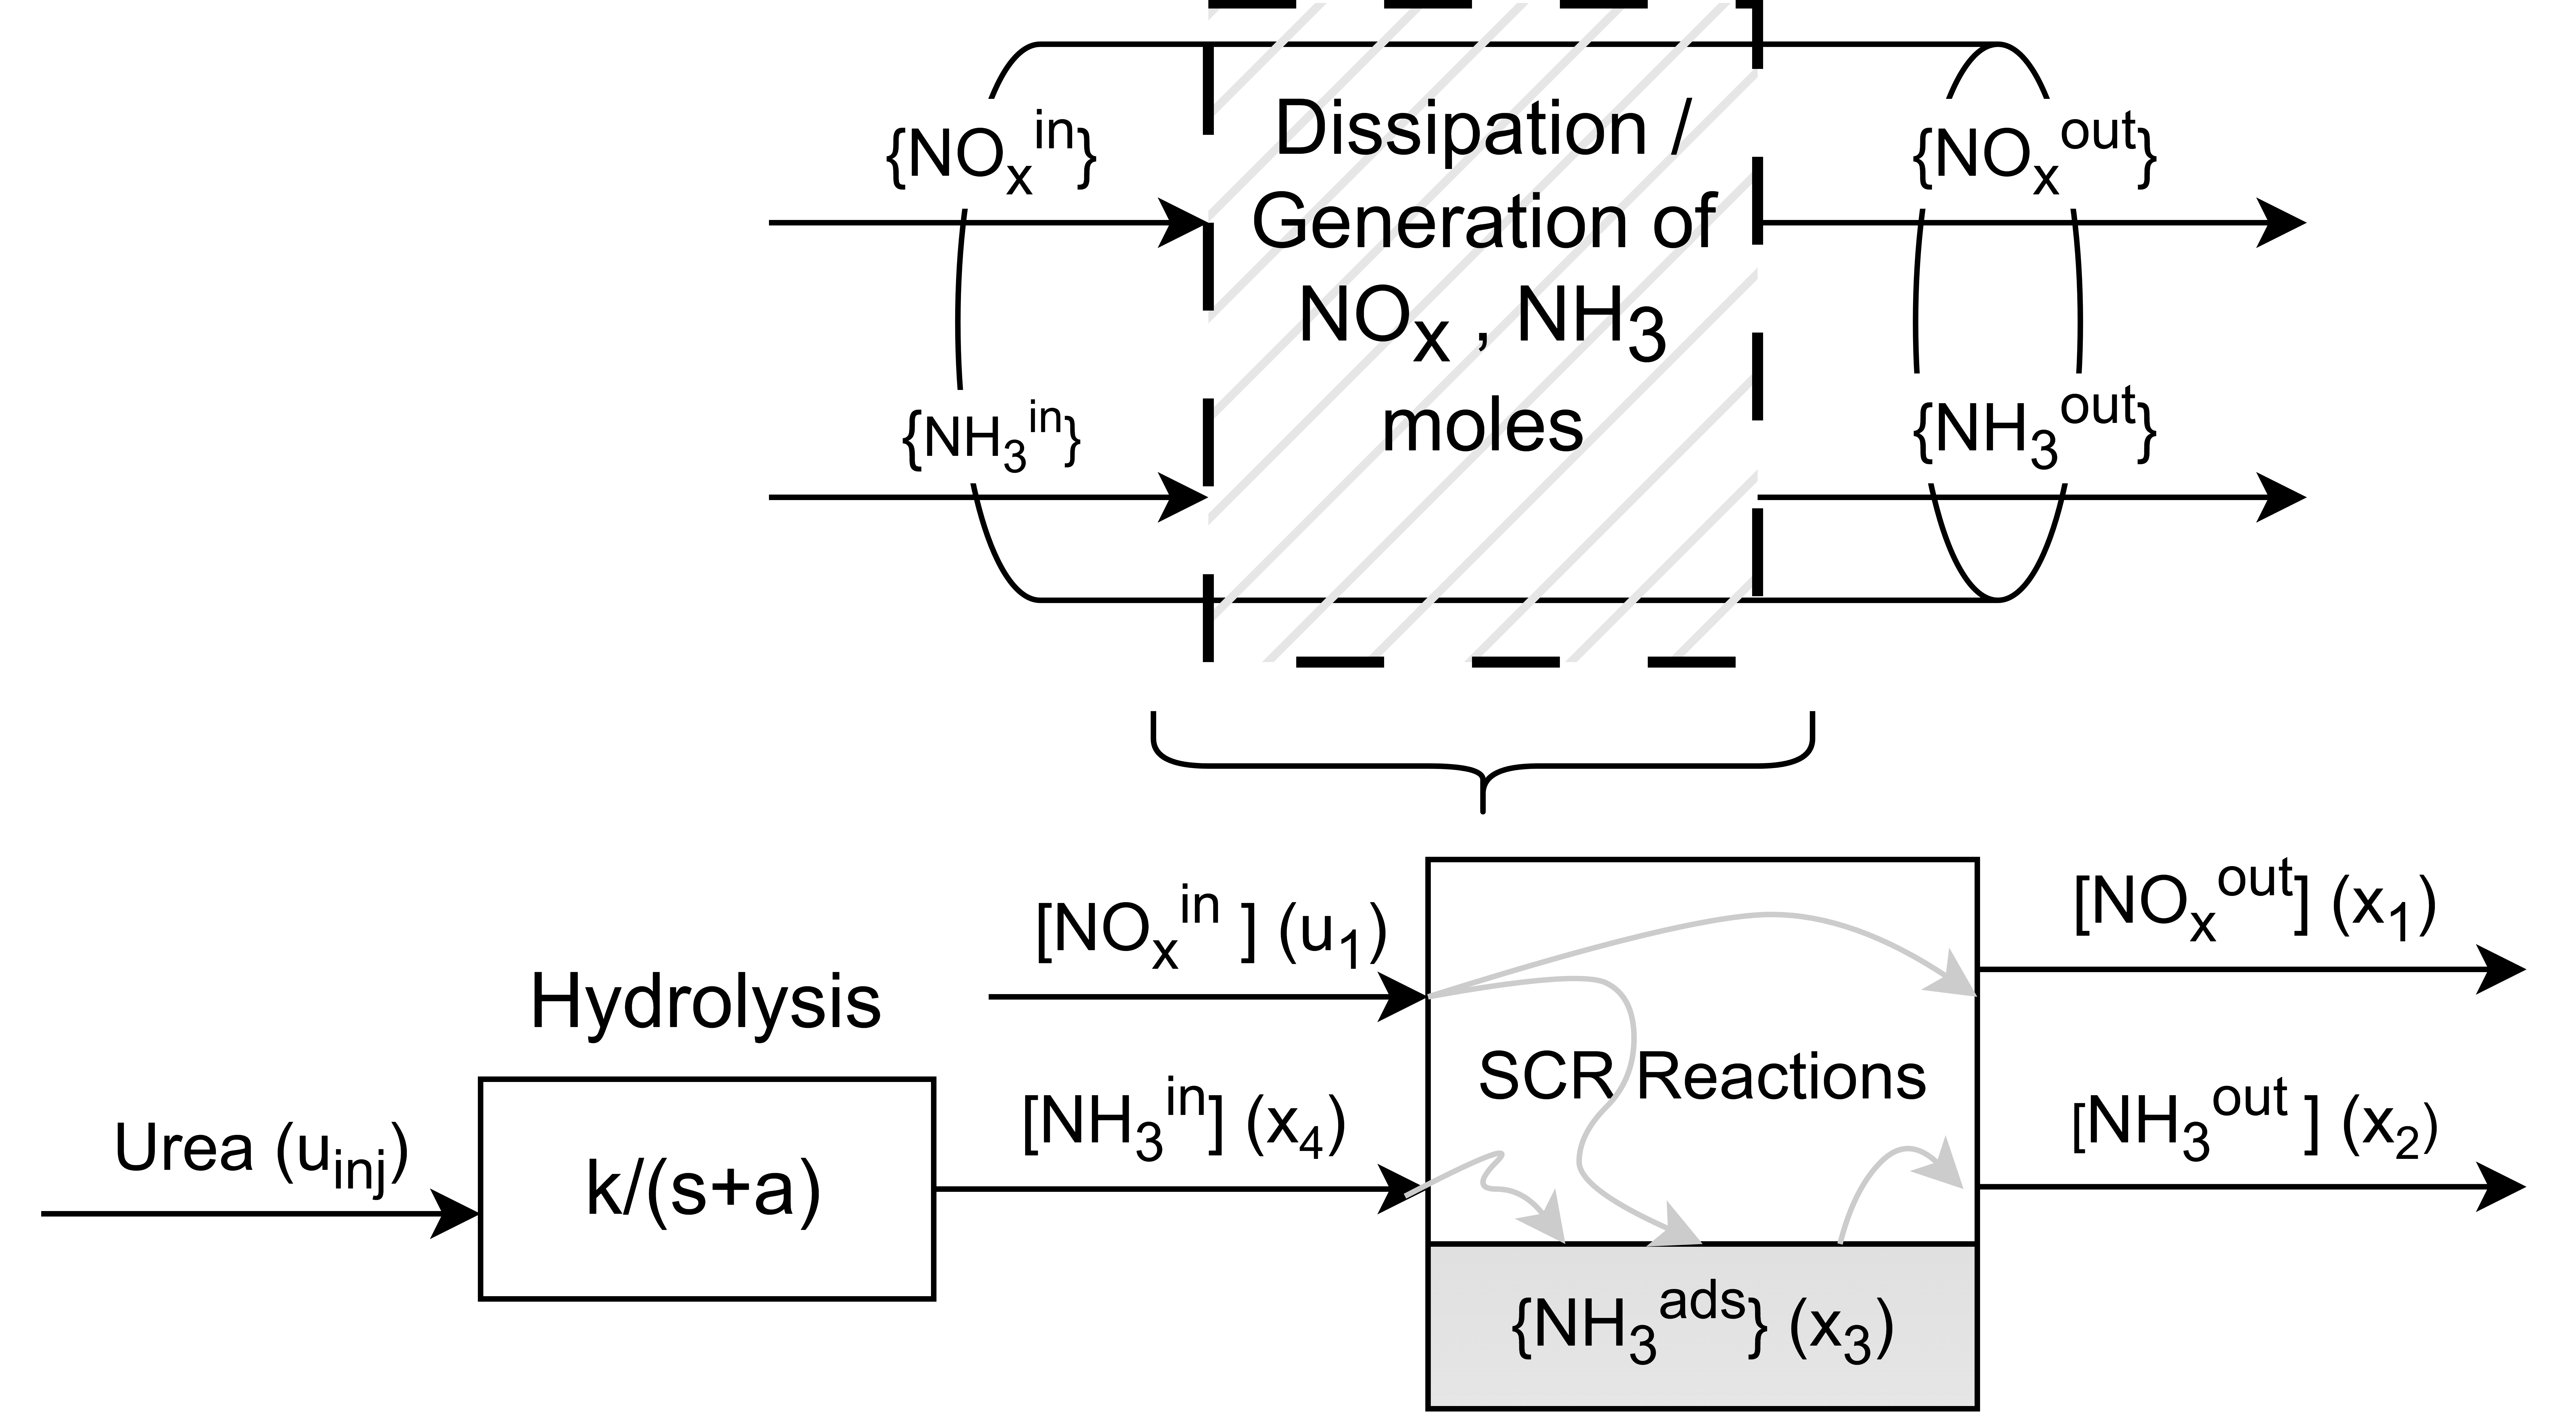
\includegraphics[width=0.45\textwidth]{./figs/scr_sys/SCR_sys.png}
    \caption{Schematic of the SCR system}
    \label{fig:exhaust_scheme}
\end{figure}


Thus, modern diesel after-treatment systems, particularly those that integrate Selective Catalytic Reduction (SCR) with
Ammonia Slip Catalyst (ASC), necessitate advanced on-board diagnostics (OBD) tools for accurate assessment of SCR
degradation levels. However, the effectiveness of traditional OBD approaches for this purpose has been impeded by the
absence of model validation with real-world catalyst degradation data and the limitations imposed by existing commercial
$NO_x$ sensors' cross-sensitivity to ammonia.

Numerous studies have been conducted on modeling the SCR-ASC systems and their control (\cite{yuan2015diesel}). A
prevalent modeling approach is to approximate the PDE model from the plug flow reactor assumption into a set of ODEs
using the idealization of the plug-flow reactor into a sequence of CSTRs (\cite{hsieh2011development}, and
\cite{nova2014urea}). This discretization requires at least 2 CSTRs to capture the system dynamics and causality,
thereby increasing the model order. Moreover, the reactions considered are generally confined to selected SCR and ASC
reactions. The single CSTR approach was first justified in \cite{devarakonda2008adequacy} and a nonlinear model was
developed using these assumptions, which was then linearized for feedback control design (\cite{devarakonda2009model}).
With this model, observers were designed to estimate the states corresponding to the catalyst's storage
(\cite{ma2017observer}, \cite{jain2020term}). A method for detecting the catalyst's aging by observing the change in the
maximum storage capacity of the catalyst, modeled as an exponential function of temperature, was also proposed in
\cite{ma2017observer}. A common theme in these studies is the resulting non-convex, nonlinear parameter estimation
problem. Moreover, these studies assume the availability of all the gaseous states at the tail-pipe to eliminate the
effects of cross-sensitivity of the $NO_x$ sensors, which is not always the case in real-world applications. One other
fundamental issue with a single cell CSTR assumption is that it results in the causality reversal at the reaction rates
as CSTR inherently assumes that the output concentrations are the same as CSTR's accumulator concentrations.


The existing models for control and estimation of diesel-engine SCR-ASC dynamics spur the need for a "low-order",
"high-fidelity" model capable of diagnostics.

One of the fundamental assumptions in the diesel engine SCR-ASC modelling, CSTR, reverts the causality in the reaction
rate constants, when the model order is reduced by considering a single cell. The present work circumvents the problem
by discarding the CSTR assumption and modelling the time evolution of the sensor signals when a "plug" or "parcel" of
the exhaust gasses flows through the chamber.

Such a time evolution introduces constraints on the model due to sampling limitations. To capture the transient
dynamics, the sampling time should be significantly smaller than the "residence time" of the reactants inside the
SCR-ASC chamber. If that is not the case as is the situation with the present available test and truck data, time integrated states assuming zero-order holds during the transients need to be introduced into the model and the input-output model can be derived from the resulting state-space model.

The modelling approach involves following the evolution of the measurement signals at the input and the output of the
system. As the plug of fluid flows through the chamber, these measurements can be correlated based on the conservation
of moles within the fluid plug.

\newpage
\section{SCR/ASC Reactions}
The following lists all the reactions that take place inside the SCR-ASC chamber.

\begin{align*}
    NH_2 - CO - NH_2 (liquid) &\longrightarrow NH_2 - CO - NH_2^* + x H_2 O
                & &[\text{AdBlue evaporation}] \\
    NH_2 - CO - NH_2^*  &\longrightarrow  HNCO + NH_3
                & &[\text{Urea decomposition}] \\
    HNCO + H_2O &\longrightarrow NH_3 + CO_2
                & &[\text{Isocynic acid hydrolysis}] \\
    %===
    NH_3 + \Theta_{free} &\leftrightharpoons NH_3(ads)
                         & &[\text{Ammonia Adsorption/Desorption}]\\
    %===
    4 NH_3 (ads) + 4 NO + O_2 &\longrightarrow 4 N_2 + 6 H_2O
                              & &[\text{Standard SCR reaction}]\\
    %===
    2 NH_3 (ads) +  NO + N O_2 &\longrightarrow 2 N_2 + 3 H_2O
                              & &[\text{Fast SCR reaction}]\\
    %===
    4 NH_3 (ads) + 3N O_2 &\longrightarrow 3.5 N_2 + 6 H_2O
                              & &[\text{Slow SCR reaction}]\\
    %===
    4 NH_3 + 3 O_2 &\longrightarrow 2 N_2 + 6 H_2O
                         & &[\text{AMOX with/without ASC}]\\
    4 NH_3 + 5 O_2 &\longrightarrow 4 NO + 6 H_2 O
                         & &[\text{AMOX with/without ASC}]\\
    2 NH_3 + 2 O_2 &\longrightarrow N_2O + 3 H_2O
                         & &[\text{AMOX with/without ASC}]\\
    %==
    2 NO + O_2 &\longrightarrow 2 NO_2
                        & &[\text{NO oxidation}]
\end{align*}

The Eley-Rideal reaction mechanism \cite{yuan2015diesel}, \cite{hsieh2011development}, \cite{nova2014urea} is considered
for interpreting the SCR reactions, where one reactant $(NO_x)$ is gaseous, and the other is adsorbed on the catalyst
surface $(NH_3)$.

Further, in order to keep the model order reasonably low, only the following three reactions are considered:
\begin{enumerate}
    \item Standard SCR reaction:
    \begin{align}
        4 NH_3 ^{ads} + 4 NO + O_2 &\xrightarrow[]{k_{scr}} 4 N_2 + 6 H_2O \label{eqn::std_scr}
    \end{align}
    \item Ammonia Oxidation:
    \begin{align}
        4 NH_3^{ads} + 3 O_2 &\xrightarrow[]{k_{oxi}} 2 N_2 + 6 H_2O \label{eqn::amox}
    \end{align}
    \item Ammonia Adsorption/Desorption:
        \begin{align}
            NH_3 + \Theta_{free} &\xrightleftharpoons[k_{des}]{k_{ads}} NH_3^{ads}
            \label{eqn::ads}
        \end{align}
\end{enumerate}


\subsection{Temperature model for rate constants}
The rate constants $(k)$ of the reactions are temperature dependent and follow the Arrhenius equation:
\begin{align*}
    k = A \exp\left(-\frac{E}{RT}\right)
\end{align*}
where $A$ is the pre-exponential factor, $E$ is the activation energy, and $R$ is the universal gas constant. The small
perturbation form of the above equation is given by:
\begin{align*}
    \delta k &= A e^{-\frac{E}{RT}} \underbrace{\lr{\frac{E}{RT^2}}}_p \delta T = k p \delta T
\end{align*}
Thus,
\begin{align*}
    k(T) \approx k(T_0) + \delta k = k(T_0) + k(T_0) p(T_0) \underbrace{\lr{T - T_0}}_{\delta T}
\end{align*}

Hence, within a certain range of temperatures, the rate constant can be assumed to be varying linearly with temperature.
Thus, the rate constant can be:
\begin{align*}
    k(T) &= mT + c \qquad  \text{for } \: T \in [T_0 - \Delta T_{max}, T_0 + \Delta T_{max}]
\end{align*}

Based on the available data, $T_0$ is chosen as $250 \lx{^o}{C}$ and $\Delta T_{max}$ such that it spans all the
available data. From linear model fitting, the validity of the linear model was found to be limited to $\pm 50
\lx{^o}{C}$.

\subsubsection{Quadratic temperature model for rate constants}
Using second-order Taylor series approximation, the expression for rate constant can be rewritten as:
\begin{align*}
    k(T) &\approx k(T_0) + k'(T_0) (T - T_0) + \frac{1}{2} k''(T_0) (T - T_0)^2\\
    \text{Let,} \qquad
    &m + 2qT_0 = k'(T_0) = \lr{\frac{AE}{RT_0^2}} e^{-\frac{E}{RT_0}} \\
    &q = k''(T_0) = \lr{\frac{A E^2}{R^2 T_0^4} - \frac{A E}{2 R T_0^3}} e^{-\frac{E}{RT_0}} \\
    \implies k(T) &\approx k(T_0) + \lr{m + 2qT_0} (T - T_0) + q (T - T_0)^2
                   = q T^2 + m T + \underbrace{\lr{ -  q T_0^2 - mT_0  + k(T_0)}}_c
\end{align*}
Thus, we can have a quadratic approximation model for the rate constant:
\begin{align}
    k(T) &= q T^2 + m T + c \qquad \text{for } \: T \in [T_0 - \Delta T_{max}, T_0 + \Delta T_{max}]
\end{align}

The subsequent derivation will use the quadratic model for the rate constant and this can be switched to linear model by setting $q = 0$.


%===============================================================================
\subsection{Model reduction: Lumping ASC reaction dynamics into SCR reaction dynamics}

\begin{figure}[H]
    \centering
    \includegraphics[width=0.9\textwidth]{./figs/scr_sys/SCR-ASC_ModelReduction_horizontal.png}
    \caption{Schematic of the SCR-ASC reduced model}
    \label{fig:scr-asc}
\end{figure}

The ammonia oxidation (AMOX) reactions are similar on SCR and ASC catalysts. First, the gaseous ammonia adsorbs onto the
catalyst system. Then, the adsorbed ammonia oxidizes into $N_2$ or $NO_x$ based on the temperature and other conditions.
As the AMOX reactions on both the catalysts are similar, it is not possible to distinguish the origin of the products
from the outlet measurements alone unless measurements between SCR and ASC sections are available.

Thus, oxidation of adsorbed ammonia on both SCR and ASC catalysts can be  combined into a single reaction, lumping the
rates constants and concentrations of the products into parameters and states of a single oxidation reaction. Further
the nitrogen selectivity of that single AMOX reaction is assumed to be $100\%$. This is valid for temperatures greater
than $225 \lx{^o}{C}$ \cite{jain2023diagnostics}, i.e., the temperature range of interest for most of the test and road
conditions.

This aggregation of reactions results in errors in the rate constant estimates, of all the SCR-ASC reactions.
Specifically, the rate constant estimate for the $NO_x$ reduction will be lower than the actual value as only a part of
the total adsorbed ammonia (on SCR catalyst) alone is involved in the reduction reaction.

\newpage
\section{Mean Residence Time}

\itbf{Definition}: Mean residence $(\tau)$ time is the average time a parcel of fluid spends inside the reactor. It is
defined as the ratio of the volume of the reactor to the volumetric flow rate of the fluid.
\begin{align}
    \tau = \frac{V}{f_v}
\end{align}

The actual residence time of the fluid inside the reactor follows a distribution based on the type of the reacting flow
(PFR, CSTR, etc) with mean as the mean residence time $(\tau)$.

For the given test-cell and truck data, the mean residence time is calculated with the following values:
\begin{align*}
    \text{Length of the chamber:}&&
    L &= L_{scr} + L_{asc} = 9.5 \, in  + 2 \, in = 11.5 \, in = 29.21 \, cm\\
    \text{Diameter of the chamber:} &&
    D &= 13 \, in = 33.02 \, cm\\
    \text{Volume of the chamber:} &&
    V &= \frac{\pi}{4} D^2 L = \frac{\pi}{4} \times 33.02^2 \times 29.21 = 25013.543 \, cm^3\\
    \text{Nominal Density:} &&
    \rho(250 \lx{^o}{C}) &= 6.75 \times 10^{-4} \, g/ml\\
    \text{Nominal Mass Flow rate:} &&
    F &= 196 \, g/s
\end{align*}
Thus, we have the mean residence time as:
\begin{align}
    \tau &= \frac{V}{f_v} = \frac{\rho V}{F} = \frac{6.75 \times 10^{-4} \times 25013.543}{196} = 0.086 \, s
\end{align}

Detailed plots of residence time calculations for the test-cell and truck data are presented in
appendix-\ref{app:res_time_plots}.
% ==============================================================================

The above calculations show that the mean residence time is around $0.1 \, s$ which is half that of the sampling time of
the test-cell data (0.2 s) and one-tenth of the sampling time ($\Delta t$) of the truck data (1 s). This implies that
the measurement signal of the gas concentrations don't capture the reaction transients that generally occur at the time
scales  that are less than the mean residence time. This also prompts us to develop an "averaged" nonlinear ARMAX model
for the system that captures the dynamics of the system at the time scales of the sampling time while capturing the
integrating (and/or memory) effects of the catalyst storage at the end of each residence time within the sample.

% ==============================================================================
\begin{table}[H]
\caption{Mean residence time of individual data sets}
\begin{minipage}{0.49\textwidth}
\begin{table}[H]
    \centering
    \begin{tabular}{r l l}
        \hline
        \hline
        \textbf{Test-cell Data} & \textbf{$\tau$ (s)} & \textbf{$\Delta t$ (s)}\\
        \hline
        \hline
        $dg\_rmc$ & 0.07 & 0.2\\
        $dg\_hftp$ & 0.16 & 0.2\\
        $dg\_cftp$ & 0.16 & 0.2\\
        $aged\_rmc$ & 0.07 & 0.2\\
        $aged\_hftp$ & 0.16 & 0.2\\
        $aged\_cftp$ & 0.16 & 0.2\\
        \hline
        \hline
    \end{tabular}
\end{table}
\end{minipage}
\begin{minipage}{0.49\textwidth}
\begin{table}[H]
    \centering
    \begin{tabular}{r l l}
        \hline
        \hline
        \textbf{Truck Data} & \textbf{$\tau$ (s)} & \textbf{$\Delta t$ (s)}\\
        \hline
        \hline
        $adt\_15$ & 0.08 & 1\\
        $adt\_17$ & 0.06 & 1\\
        $mes\_15$ & 0.1 & 1\\
        $mes\_18$ & 0.08 & 1\\
        $trw\_15$ & 0.09 & 1\\
        $trw\_18$ & 0.08 & 1\\
        $wer\_15$ & 0.08 & 1\\
        $wer\_17$ & 0.09 & 1\\
        \hline
        \hline
    \end{tabular}
\end{table}
\end{minipage}
\end{table}

\newpage
\section{Ammonia Adsorption/Desorption Process Dynamics}
\begin{figure}[H]
    \centering
    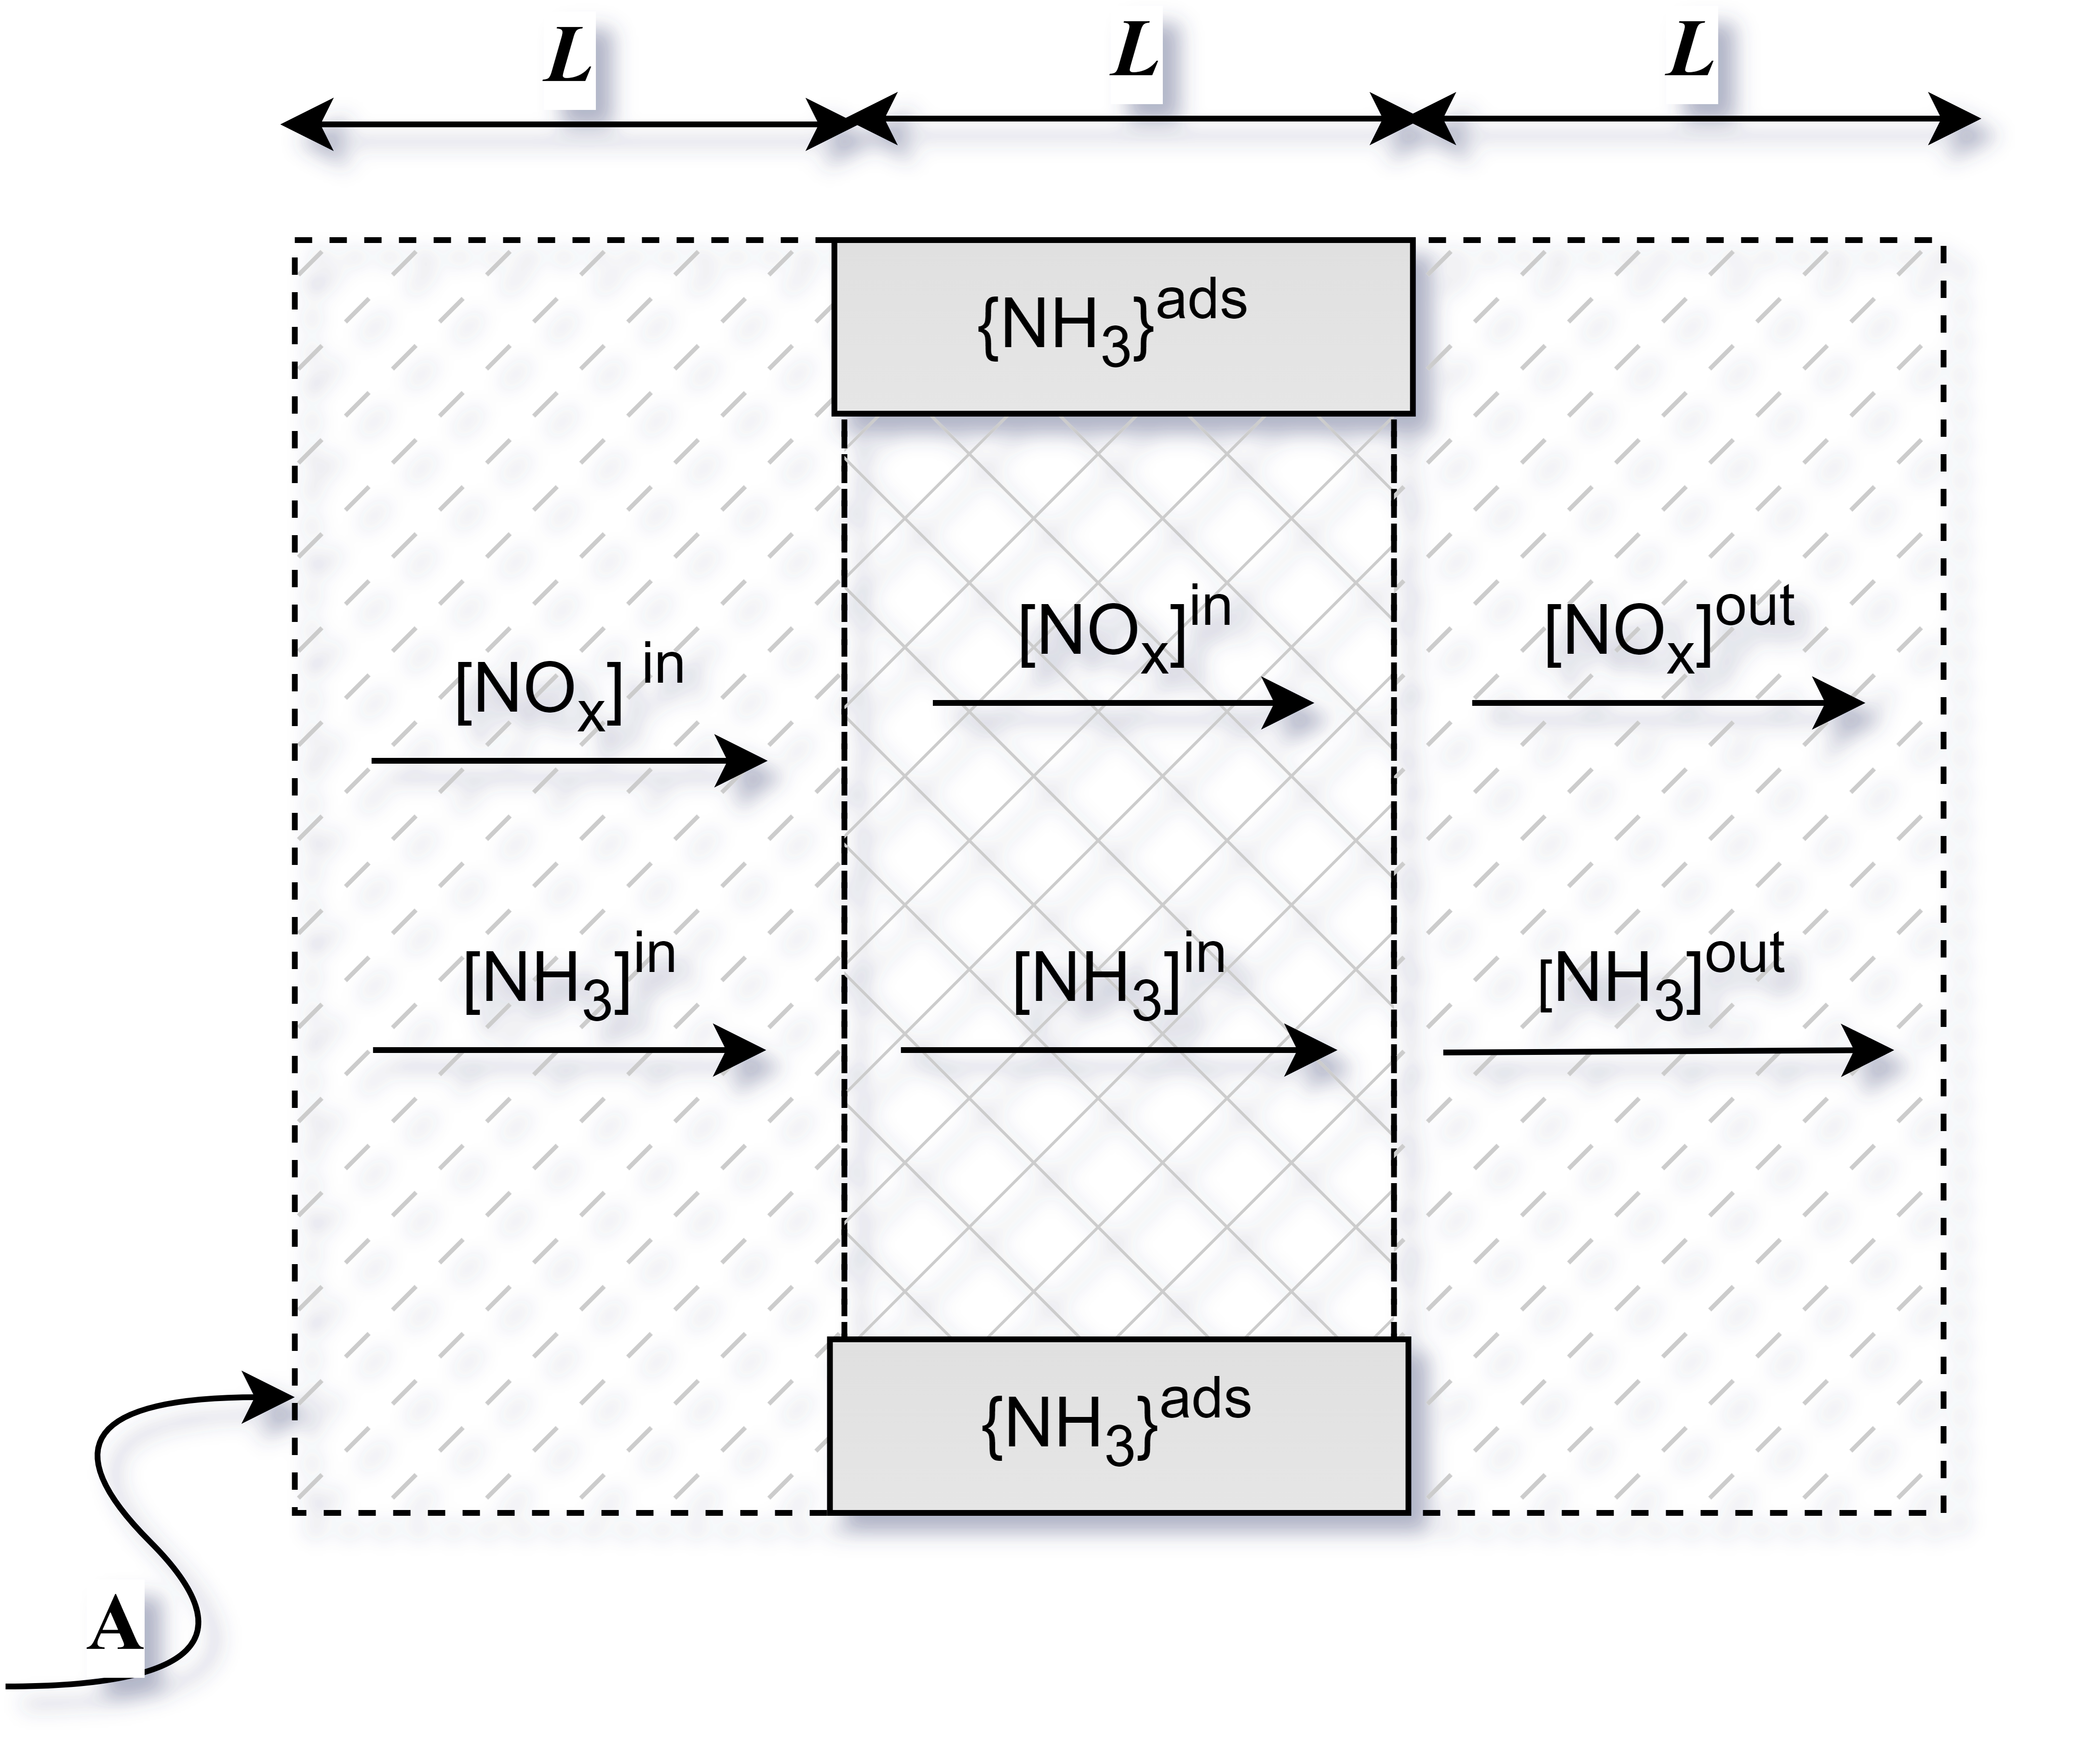
\includegraphics[width=0.5\textwidth]{./figs/scr_sys/plug_flow_discrete.png}
    \caption{Discrete plug-flow reactor model}
    \label{fig:plug_flow_discrete}
\end{figure}
%===
The ammonia adsorption/desorption process dynamics involve all the three above-mentioned reactions. The gaseous ammonia
that enters the catalyst chamber gets adsorbed onto the free sites on the catalyst surface at a rate proportional to the
volumetric concentration of the gaseous ammonia and the surface concentration of the free sites. The adsorbed ammonia
then either reacts with the gaseous $NO_x$ (Eiley-Rideal Mechanism) releasing $N_2$ and $H_2O$ or decomposes to form
$N_2$ and $H_2O$ (Surface Decomposition). In either case, the process frees up the adsorption sites for the next cycle
of gaseous ammonia.
%===
\begin{align*}
    4 NH_3 ^{ads} + 4 NO + O_2 &\xrightarrow[]{k_{scr}} 4 N_2 + 6 H_2O \\
    4 NH_3^{ads} + 3 O_2 &\xrightarrow[]{k_{oxi}} 2 N_2 + 6 H_2O \\
    NH_3 + \Theta_{free} &\xrightleftharpoons[k_{des}]{k_{ads}} NH_3^{ads}
\end{align*}
Thus, the rate of ammonia adsorption on the catalyst surface can be modeled as:
\begin{align*}
    \frac{d \con{NH_3}^{ads}}{dt} &= r_{ads} - r_{des} - r_{scr} - r_{oxi}\\
    r_{ads} &= k_{ads} \con{NH_3}^{in} \lr{\Gamma - \con{NH_3}^{ads}} \qquad \lrb{\Gamma = \frac{\Theta_{free} + \Theta_{occupied}}{A_{scr}}}\\
    r_{des} &= k_{des} \con{NH_3}^{ads}\\
    r_{scr} &= k_{scr} \con{NH_3}^{ads} \con{NO_x}^{in}\\
    r_{oxi} &= k_{oxi} \con{NH_3}^{ads}\\
    \dot{\con{NH_3}}^{ads} &= \Gamma \underbrace{k_{ads} \con{NH_3}^{in}}_{\gamma_{ads}} - \con{NH_3}^{ads} \underbrace{\lr{k_{ads} \con{NH_3}^{in} + k_{des} + k_{scr} \con{NO_x}^{in} + k_{oxi}}}_{\gamma_{des}}
\end{align*}
\itbf{Note:} $\Gamma$ and $\con{NH_3}^{ads}$ are surface concentrations (in $moles/cm^2$) while the rest are volumetric
concentrations (in $moles/cm^3$). The rate constant units are adjusted appropriately to make the rate equations
consistent.

The units of all the rates and rate constants are tabulated below:
\begin{align*}
    r_{ads} &= \frac{moles}{cm^2 \cdot s} &
    k_{ads} &= \frac{cm^3}{moles \cdot s} \\
    r_{des} &= \frac{moles}{cm^2 \cdot s} &
    k_{des} &= s^{-1} \\
    r_{scr} &= \frac{moles}{cm^2 \cdot s} &
    k_{scr} &= \frac{cm^3}{moles \cdot s} \\
    r_{oxi} &= \frac{moles}{cm^2 \cdot s} &
    k_{oxi} &= s^{-1}
\end{align*}
%===
\itbf{Note:}In this section we are interested in the Surface rates where the products are assumed to linger just on the
surface of the catalyst. The surface rates of the gaseous products/reactants can be converted to volumetric rates by
using the conversion factor $A_{scr}/V$ where $A_{scr}$ is the area of the SCR catalyst and V is the volume of the
catalyst chamber. This assumes that there is instantaneous mixing of the close-to-surface moles with the gaseous moles.
Thus,
\begin{align}
    k^{vol} = \underbrace{\lr{\frac{A_{scr}}{V}}}_{k_{s2v} \, (cm^{-1})} k^{surf}
\end{align}
% ==============================================================================
\subsection{Molar conservation at the scale of residence time}

The molar storage on the catalyst surface changes at the end of every residence time and a "fresh" set of gaseous
reactants enters the catalyst chamber. And, within the sample time $t_s$, the volumetric concentrations of the gaseous
reactants can be considered constant. \itbf{Let there be $n$ residence times within one sample time.} It is implicitly
assumed that there are integer number of residence times within one sample time. When that is not the case, the
resulting is error is attributed to model structure error.
\begin{align}
    t_s &= n \tau
    \label{eqn::ts_2_tau}
\end{align}

Noting that $\lrf{\bullet}$ denotes moles and $\lrb{\bullet}$ denotes the concentration of the species, the molar conservation for the adsorption/desorption process can be written as:

\begin{align*}
    \mol{NH_3}^{ads} (k + \tau) &= \mol{NH_3}^{ads} (k) + A_{scr} \int_{0}^{\tau} \dot{\con{NH_3}}^{ads} (k) dt\\
    \mol{NH_3}^{ads} (k + 2\tau) &= \mol{NH_3}^{ads} (k + \tau) + A_{scr} \int_{0}^{\tau} \dot{\con{NH_3}}^{ads} (k + \tau) dt\\
    \vdots&\\
    \mol{NH_3}^{ads} (k + n\tau) &= \mol{NH_3}^{ads} (k + (n-1)\tau) + A_{scr} \int_{0}^{\tau} \dot{\con{NH_3}}^{ads} (k + (n-1)\tau) dt
\end{align*}

\begin{align*}
    \mol{NH_3}^{ads}(k + 1) = \mol{NH_3}^{ads} (k + n\tau) &= \mol{NH_3}^{ads} (k) + A_{scr} \sum_{i=0}^{n-1} \int_{0}^{\tau} \dot{\con{NH_3}}^{ads} (k + i\tau) dt
\end{align*}

Writing the above equation in terms of surface concentrations:
\begin{align*}
    \con{NH_3}^{ads}(k + 1) = \con{NH_3}^{ads} (k + n\tau) &= \con{NH_3}^{ads} (k) + \underbrace{\sum_{i=0}^{n-1} \int_{0}^{\tau} \dot{\con{NH_3}}^{ads} (k + i\tau)}_{\Omega(k)}   dt
\end{align*}

$\Omega(k)$ is the total change in the surface concentration of adsorbed ammonia
within one sample time.

% ==============================================================================
\subsection{Calculating the total surface concentration change of adsorbed ammonia within one sample time $\Omega(k)$}

The volumetric concentrations of the gaseous reactants are assumed to be
constant within the sample time, while the surface concentrations change at the
end of every residence time.

\begin{align*}
    \dot{\con{NH_3}}^{ads} (k + i\tau) &= r_{ads} (k + i \tau) - r_{des} (k + i \tau) - r_{scr} (k + i \tau) - r_{oxi} (k + i \tau)\\
    %===
    r_{ads} (k + i \tau) &= k_{ads} \con{NH_3}^{in}(k) \lr{\Gamma - \con{NH_3}^{ads} (k + i \tau)}\\
    r_{des} (k + i \tau) &= k_{des} \con{NH_3}^{ads}(k + i \tau)\\
    r_{scr} (k + i \tau) &= k_{scr} \con{NH_3}^{ads}(k + i \tau) \con{NO_x}^{in}(k)\\
    r_{oxi} (k + i \tau) &= k_{oxi} \con{NH_3}^{ads}(k + i \tau)\\
    \gamma_{ads} (k) &= k_{ads} \con{NH_3}^{in}(k)\\
    \gamma_{des} (k) &= \lr{k_{ads} \con{NH_3}^{in}(k) + k_{des} + k_{scr} \con{NO_x}^{in}(k) + k_{oxi}}\\
    %===
    \dot{\con{NH_3}}^{ads} (k + i\tau) &= \Gamma \gamma_{ads} (k) - \con{NH_3}^{ads} (k + i \tau) \gamma_{des} (k)
\end{align*}

Calculating the expression for $\Omega(k)$:
\begin{align*}
    \Omega(k) &= \sum_{i=0}^{n-1} \int_{0}^{\tau} \dot{\con{NH_3}}^{ads} (k + i\tau) dt\\
    &= \sum_{i=0}^{n-1} \dot{\con{NH_3}}^{ads} (k + i\tau) \tau \qquad \lrb{\because \text{The rate is assumed to be constant within the residence time}}\\
    &= \sum_{i=0}^{n-1} \lr{\Gamma \gamma_{ads} (k) - \con{NH_3}^{ads} (k + i \tau) \gamma_{des} (k)} \tau\\
    &= \tau n \Gamma \gamma_{ads} (k) - \tau \gamma_{des} (k) \underbrace{\sum_{i=0}^{n-1} \con{NH_3}^{ads} (k + i \tau) }_{n \sigma(k)} \\
    &= n \tau \lr{\Gamma \gamma_{ads} (k) - \sigma(k) \gamma_{des} (k)}
\end{align*}

The term $\sigma(k)$ is unknown and unobservable. It is the average surface
concentration at the end of every residence time within the sample time.

Moreover, we can get the expression for average rate of change of the surface
concentrations within the sample time as:
\begin{align*}
    \dot{\con{NH_3}}^{ads} (k) &= \frac{\Omega(k)}{\tau n} = \Gamma \gamma_{ads} (k) - \sigma(k) \gamma_{des} (k)\\
    &= \Gamma k_{ads} \con{NH_3}^{in}(k) - \sigma(k) \lr{k_{ads} \con{NH_3}^{in}(k) + k_{des} + k_{scr} \con{NO_x}^{in}(k) + k_{oxi}}
\end{align*}

% ==============================================================================

\subsection{Ammonia adsorption/desorption process dynamics model}
Substituting the expression for $\Omega(k)$ in the equation for
$\con{NH_3}^{ads}(k + 1)$:

\begin{align*}
    \con{NH_3}^{ads}(k + 1) &= \con{NH_3}^{ads} (k) + n \tau \lr{\Gamma \gamma_{ads} (k) - \sigma(k) \gamma_{des} (k)}\\
    &= \con{NH_3}^{ads}(k) + n \tau \Gamma k_{ads} \con{NH_3}^{in}(k) - n \tau \sigma(k) \lr{k_{ads} \con{NH_3}^{in}(k) + k_{des} + k_{scr} \con{NO_x}^{in}(k) + k_{oxi}}
\end{align*}

\subsection{Approximation of $\sigma(k)$ as $NH_3^{ads}(k)$ (Zero-order hold)}
\itbf{Note:} $\sigma(k)$ can be approximated as the surface concentration at the beginning of the sample time.

The average surface concentration $\sigma(k)$ in the sample time is approximated
as the surface concentration at the beginning of the sample time. This
approximation will introduce an error in the model whose effects will be
analyzed in sequential sections.

Thus,
\begin{align}
    \Omega(k) &\approx n \tau \lr{\Gamma \gamma_{ads} (k) - \con{NH_3}^{ads}(k) \gamma_{des} (k)}
\end{align}

Thus, we have approximate ammonia adsorption/desorption process dynamics model as:

\begin{align*}
    \con{NH_3}^{ads}(k + 1) &= \con{NH_3}^{ads} (k) + n \tau \lr{\Gamma \gamma_{ads} (k) - \con{NH_3}^{ads}(k) \gamma_{des} (k)}\\
    &= n \tau \Gamma \gamma_{ads} (k) + \con{NH_3}^{ads} (k) \lr{1 - n \tau \gamma_{des} (k)}\\
    &= n \tau \Gamma k_{ads} \con{NH_3}^{in}(k)  + \con{NH_3}^{ads} (k) \lr{1 - n \tau \lr{k_{ads} \con{NH_3}^{in}(k) + k_{des} + k_{scr} \con{NO_x}^{in}(k) + k_{oxi}}}
\end{align*}


\begin{align}
    \con{NH_3}^{ads}(k + 1) &= n \tau \Gamma k_{ads} \con{NH_3}^{in}(k)  + \con{NH_3}^{ads} (k) \lr{1 - n \tau \lr{k_{ads} \con{NH_3}^{in}(k) + k_{des} + k_{scr} \con{NO_x}^{in}(k) + k_{oxi}}}
\end{align}

Examining the individual terms:
\begin{align*}
    \con{NH_3}^{ads}(k + 1) =& \con{NH_3}^{ads}(k)\\
        &+ n\tau k_{ads} \con{NH_3}^{in} \lr{\Gamma - \con{NH_3}^{ads}(k)} \\
        &- n \tau \lr{k_{oxi} + k_{des}} \con{NH_3}^{ads} (k)\\
        &- n \tau k_{scr} \con{NO_x}^{in}(k) \con{NH_3}^{ads}(k)
\end{align*}

The above equation is nothing but multiplying the rate equation with the
sampling interval to get the measurement update.

Similarly, if we flip the approximation, that is if,
\begin{align*}
    \con{NH_3}^{ads}(k) &\approx \sigma(k)
\end{align*}
then,

\begin{align*}
    \sigma(k + 1) =& \sigma(k)\\
        &+ n\tau k_{ads} \con{NH_3}^{in} \lr{\Gamma - \sigma(k)} \\
        &- n \tau \lr{k_{oxi} + k_{des}} \sigma(k)\\
        &- n \tau k_{scr} \con{NO_x}^{in}(k) \sigma(k)
\end{align*}


\newpage
\section{$NO_x$ Process Dynamics}

The $NO_x$ process dynamics involve only the selective catalytic reduction
reaction. The gaseous $NO_x$ that enters the catalyst chamber reacts with the
adsorbed ammonia on the surface and forms $N_2$ and $H_2O$ (Eiley-Rideal
Mechanism). The process frees up the adsorption sites for the next cycle of
gasueous ammonia. The reaction reate is proportional to the volumetric concentration of the gaseous $NO_x$ and the surface concentration of the adsorbed ammonia.

\begin{align}
    4 NH_3 ^{ads} + 4 NO + O_2 &\xrightarrow[]{k_{scr}} 4 N_2 + 6 H_2O
\end{align}


Thus, the rate of $NO_x$ reduction on the catalyst surface can be modeled as:

\begin{align}
    \frac{d \con{NO_x}^{scr}}{dt} &= - k_{s2v} r_{scr} \\
    r_{scr} &= k_{scr} \con{NH_3}^{ads} \con{NO_x}^{in}\\
    \dot{\con{NO_x}}^{scr} &= -k_{s2v} k_{scr} \con{NH_3}^{ads} \con{NO_x}^{in}
\end{align}

% ==============================================================================

\subsection{Molar conservation at the scale of residence time}

Similar to the ammonia adsorption/desorption process, at the end of every
residence time, a fresh parcel of gaseous reactants enters the catalyst
chamber. Thus, the molar conservation for the $NO_x$ reduction process can be
will correlate the inlet and outlet molar concentrations of the $NO_x$ at the
beginning and the end of residence time. Thus,

\begin{align*}
    \mol{NO_x}^{out} (k + \tau) &= \mol{NO_x}^{in} (k) + V \int_{0}^{\tau}  \dot{\con{NO_x}}^{scr} (k) dt\\
    \mol{NO_x}^{out} (k + 2\tau) &= \mol{NO_x}^{in} (k + \tau) + V \int_{0}^{\tau} \dot{\con{NO_x}}^{scr} (k+\tau)  dt\\
    \vdots &\\
    \mol{NO_x}^{out} (k + n\tau) &= \mol{NO_x}^{in} (k + (n-1)\tau) + V \int_{0}^{\tau} \dot{\con{NO_x}}^{scr} (k+(n-1)\tau) dt
\end{align*}

The above equations show that the measurement of $NO_x$ concentration at the
outlet depends only on the measurement of the $NO_x$ concentration at the inlet
on residence time before. Thus, there is no integrating effect of the $NO_x$
within the sample time. Writing interms of volumetric concentrations, we have:

\begin{align*}
    \con{NO_x}^{out} (k + n\tau) &= \con{NO_x}^{in} (k + (n-1)\tau) + \int_{0}^{\tau}  \dot{\con{NO_x}}^{scr} (k + (n-1)\tau) dt
\end{align*}

Introducing the following two approximation:
\begin{enumerate}
    \item Zero-order-hold for the inlet concentration of $NO_x$:
        \begin{align*}
            \con{NO_x}^{in} (k + i \tau) &\approx \con{NO_x}^{in} (k) \qquad \forall i < n
        \end{align*}
    \item Using average surface concentration at the sample for the surface concentration of the adsorbed ammonia:
        \begin{align*}
            \con{NH_3}^{ads} (k + i \tau) &\approx \sigma(k) \qquad \forall i < n
        \end{align*}
\end{enumerate}

Thus,
\begin{align*}
    \dot{\con{NO_x}}^{scr} (k + i \tau) =  \dot{\con{NO_x}}^{scr} (k) = -k_{s2v} k_{scr} \sigma(k) \con{NO_x}^{in} (k) \qquad \forall i < n
\end{align*}


Thus, we have the following expression for the $NO_x$ process dynamics:

\begin{align*}
    \con{NO_x}^{out} (k + n\tau) &= \con{NO_x}^{in} (k) - k_{s2v} k_{scr} \sigma(k) \con{NO_x}^{in} (k) \tau\\
    \implies \con{NO_x}^{out} (k + 1) &= \con{NO_x}^{in} (k) \lr{1 - k_{s2v} k_{scr} \sigma(k) \tau}
\end{align*}


% ==============================================================================

\subsection{Preliminary aging signature}
The $NO_x$ process dynamics can be rewritten as:
\begin{align*}
    \frac{\con{NO_x}^{in}(k) - \con{NO_x}^{out}(k + 1)}{\con{NO_x}^{in}(k)} &=
    k_{s2v} k_{scr} \sigma(k) \tau\\
    &= \frac{A_{scr}}{V} \times k_{scr} \times \sigma(k) \lr{\frac{V \rho}{F}}\\
    %===
    \implies F \lr{\frac{\con{NO_x}^{in}(k) - \con{NO_x}^{out}(k + 1)}{\con{NO_x}^{in}(k)}} &= \lr{\rho A_{scr} k_{scr}} \sigma(k) \\
    %===
\end{align*}

Using the linear assumption for temperature dependence of the rate constant, and
ideal gas-law for density, let:
\begin{align*}
    k_{scr} &= m_{scr} T + c_{scr}\\
    \rho &= \frac{\mu}{T}
\end{align*}
T is in Kelvin.
\begin{align*}
    \implies \underbrace{\lr{\mu A_{scr} m_{scr}}\sigma}_{\alpha_1(k)}  T+ \underbrace{\lr{\mu A_{scr} c_{scr}} \sigma}_{\alpha_0(k)} &= \underbrace{T F \lr{\frac{\con{NO_x}^{in}(k) - \con{NO_x}^{out}(k + 1)}{\con{NO_x}^{in}(k)}}}_{\beta(k)}
\end{align*}

Thus, $\alpha_1(k)$ and $\alpha_0(k)$ are monotonic first order
polynomials in $\sigma$. Assuming, the average surface concentration of ammonia
on the catalyst is higher for degreened catalyst than for aged catalyst, we can
use $\alpha_1, \alpha_0$ to define a preliminary aging signature for the
catalyst. This can be used to monitor the aging of the catalyst in real-time.


The variables, $\alpha_1(k)$ and $\alpha_0(k)$ change with time. The only way to
estimate these variables is to estimate a moving-averaged version of it.


% ==============================================================================
We have the above equation for $n$ (Averaging window) samples:

\begin{align*}
    \alpha_1(k) T(k) + \alpha_0(k) &= \beta(k)\\
    \alpha_1(k-1)T(k-1) + \alpha_0(k-1) &= \beta(k-1)\\
    \vdots &\\
    \alpha_1(k-(n-1))T(k-(n-1)) + \alpha_0(k-(n-1)) &= \beta(k-(n-1))\\
\end{align*}

Let,
\begin{align*}
    \bar \alpha_1(k) &= \frac{1}{n} \sum_{i=0}^{n-1} \alpha_1(k-i)\\
    \bar \alpha_0(k) &= \frac{1}{n} \sum_{i=0}^{n-1} \alpha_0(k-i)\\
\end{align*}

Thus, we have the following equation:
\begin{align*}
    \bm{\bar \alpha_1(k)\\
        \bar \alpha_0(k)} &=
        \bm{T(k) & 1\\
            T(k-1) & 1\\
            \vdots & \vdots\\
            T(k-(n-1)) & 1}^{-1}
        \bm{\beta(k)\\
            \beta(k-1)\\
            \vdots\\
            \beta(k-(n-1))}
\end{align*}


\newpage
\section{Gaseous Ammonia Process Dynamics}
The gaseous ammonia process dynamics involve the adsorption and desorption dynamics. The gaseous ammonia that enters the
catalyst chamber gets adsorbed on the free sites on the catalyst surface at a rate proportional to the volumetric
concentration of the gaseous ammonia and the surface concentration of the free sites. A part of adsorbed ammonia then
desorbs back to the gas phase at a rate that is proportional to the surface concentrations of the adsorbed ammonia.
\begin{align*}
    NH_3 + \Theta_{free} &\xrightleftharpoons[k_{des}]{k_{ads}} NH_3^{ads}
\end{align*}

Thus, the rate of change of gaseous $NH_3$ on the catalyst surface can be modeled as:
\begin{align*}
    \frac{d \con{NH_3}^{scr}}{dt} &= k_{s2v} (-r_{ads} + r_{des}) \\
    r_{ads} &= k_{ads} \con{NH_3}^{in} \lr{\Gamma - \con{NH_3}^{ads}}\\
    r_{des} &= k_{des} \con{NH_3}^{ads}\\
    \dot{\con{NH_3}}^{scr} &= -k_{s2v}k_{ads} \con{NH_3}^{in} \lr{\Gamma - \con{NH_3}^{ads}} + k_{s2v} k_{des} \con{NH_3}^{ads}\\
\end{align*}

% ==============================================================================
\subsection{Molar conservation at the scale of residence time}

Similar to the ammonia adsorption/desorption process, at the end of every residence time, a fresh parcel of gaseous
reactants enters the catalyst chamber. Thus, the molar conservation for the gaseous $NH_3$ adsorption/desorption process
can be correlated with the inlet and outlet molar concentrations of the $NH_3$ at the beginning and the end of residence
time. Similar to the $NO_x$ process dynamics the measurement of $NH_3$ concentration at the outlet depends only on the
measurement of the $NH_3$ concentration at the inlet one residence time before. That is, there is no integrating effect
of the $NH_3$ within the sample time either. Writing in terms of volumetric concentrations, we have:

\begin{align*}
    \con{NH_3}^{out} (k + n\tau) &= \con{NH_3}^{in} (k + (n-1)\tau) + \int_{0}^{\tau}  \dot{\con{NH_3}}^{scr} (k + (n-1)\tau) dt
\end{align*}

Introducing the following two approximations:
\begin{enumerate}
    \item Zero-order-hold for the inlet concentration of $NH_3$:
        \begin{align*}
            \con{NH_3}^{in} (k + i \tau) &\approx \con{NH_3}^{in} (k) \qquad \forall i < n
        \end{align*}
    \item Using average surface concentration at the sample for the surface concentration of the adsorbed ammonia:
        \begin{align*}
            \con{NH_3}^{ads} (k + i \tau) &\approx \sigma(k) \qquad \forall i < n
        \end{align*}
\end{enumerate}

Thus,
\begin{align*}
    \dot{\con{NH_3}}^{scr} (k + i \tau) &= -k_{s2v}k_{ads} \con{NH_3}^{in} \lr{\Gamma - \sigma(k)} + k_{s2v} k_{des} \sigma(k)
    \qquad \forall i < n
\end{align*}


Thus, we have the following expression for the $NH_3$ process dynamics:

\begin{align*}
    \con{NH_3}^{out} (k + n\tau) &= \con{NH_3}^{in} (k) - \tau k_{s2v}k_{ads} \con{NH_3}^{in}(k) \lr{\Gamma - \sigma(k)} + \tau k_{s2v} k_{des} \sigma(k)\\
    \con{NH_3}^{out} (k + 1) &= \con{NH_3}^{in}(k) \lr{1 - \tau k_{s2v}k_{ads} \lr{\Gamma - \sigma(k)}} + \tau k_{s2v} k_{des} \sigma(k)
\end{align*}

\newpage
\section{Urea Dosing Process Dynamics}
The urea dosing dynamics involve the following reactions:
\begin{align*}
    NH_2 - CO - NH_2 (liquid) &\longrightarrow NH_2 - CO - NH_2^* + x H_2 O
                & &[\text{AdBlue evaporation}] \\
    NH_2 - CO - NH_2^*  &\longrightarrow  HNCO + NH_3
                & &[\text{Urea decomposition}] \\
    HNCO + H_2O &\longrightarrow NH_3 + CO_2
                & &[\text{Isocynic acid hydrolysis}] \\
\end{align*}

The above reactions can be aggregated into:
\begin{align*}
    NH_2 - CO - NH_2 (liquid) &\longrightarrow 2 NH_3 + CO_2 + x H_2 O
\end{align*}

The rate of ammonia production is twice the rate of decomposition of the urea in the solution (AdBlue). Thus,
\begin{align*}
    \frac{d \con{NH_3}^{in}}{dt} &= 2 r_{u}\\
    r_{u} &= k_{u} \con{NH_2 - CO - NH_2} \qquad (constant)
\end{align*}

As the concentration of urea in the solution is constant, the above rate becomes a constant. Thus, the total moles of
ammonia produced at the inlet within a sample time would be:
\begin{align*}
    \mol{NH_3}^{in} (k) &= t_s \times \underbrace{2 r_{u}}_{\text{Rate of decomposition}} \times \underbrace{t_s u_{inj} (k)}_{\text{Volume injected}}
\end{align*}
Where $u_{inj}$ urea-solution injection rate in $ml/s$.

This is the total moles of ammonia produced in $n$ residence times during the reaction process. Thus, the number of moles of ammonia in the chamber at a given residence time would be $\mol{NH_3}^{in}(k)/n$.
Thus, we have the inlet volumetric concentration of ammonia as:
\begin{align*}
    \con{NH_3}^{in} (k) &= \frac{\mol{NH_3}^{in} (k)}{nV}
                          = \frac{2 r_u \tau}{t_s V} \times t_s^2 \times u_{inj} (k)
                          = \frac{2 r_u t_s}{V} \times \tau \times u_{inj} (k)
\end{align*}
Thus the ammonia concentration at the inlet is a function of urea dosing rate and the residence time of the reaction.

Substituting, $\tau = \frac{V \rho_0}{F}$, we get:
\begin{align}
    \con{NH_3}^{in} (k) &= 2r_u t_s \rho_0 \times \frac{u_{inj}(k)}{F}
\end{align}

The above reciprocal relationship breaks down at zero flow rate which makes sense physically.

% ======================================================================================================================
The sensitivity of change in ammonia to the change residence time (due to change in flow-rate) or change in urea dosing rate can be calculated as follows:
\begin{align*}
    \frac{\partial \con{NH_3}^{in} }{\partial F} &= -2 r_u t_s \rho_0 \times \frac{u_{inj}}{F^2} \\
    \implies \frac{\delta \con{NH_3}^{in}}{\con{NH_3}^{in}} &= \frac{-\delta F}{F}
    \qquad \text{at constant } u_{inj}
\end{align*}
Similarly,
\begin{align*}
    \frac{\partial \con{NH_3}^{in} }{\partial u_{inj}} &= \frac{2 r_u t_s \rho_0}{F} \\
    \implies \frac{\delta \con{NH_3}^{in}}{\con{NH_3}^{in}} &= \frac{ \delta u_{inj}}{u_{inj}} \qquad \text{at constant } F
\end{align*}

From practical ranges changes in data for $F$ and $u_{inj}$,
\begin{align*}
    \frac{ \delta u_{inj}}{u_{inj}}, \qquad \frac{\delta F}{F} \qquad \text{have the same order of magnitude.}
\end{align*}
Thus, the effect of change in the urea dosing is as prominent on inlet ammonia concentration as the changes in residence time due to flow rate changes. Thus, the effects of changes in residence time on ammonia generation can be neglected for the approximate model, resulting in:
\begin{align}
    \con{NH_3}^{in}(k) &= \nu_u \frac{u_{inj}}{F}    \label{eqn::urea_inj}
\end{align}
where,
\begin{align*}
    \nu_u &= 2 r_u t_s \rho_0\\
    T_{min} &\leq T \leq T_{max}\\
    F_{min} &\leq F \leq F_{max}
\end{align*}

\newpage
\section{Data Interpretation}
The available test and truck data for testing the model structure needs to be
got into common units. The following table lists the units used for each
of the physical property.
\begin{align*}
    \text{Property}\quad       & \text{Unit} \\
    \text{concentration}: \quad & mol/cm^{3} = mol/ml \\
    \text{temperature}:\quad    & \lx{^o}{C} \\
    \text{time}:\quad           & s \\
    \text{mass}:\quad           & g \\
    \text{lenght}:\quad         & cm \\
\end{align*}

The data available and corresponding units are listed in the following table.

\begin{table}[H]
\centering
\begin{tabular}{l l l }
\hline \hline
Model Variable & Road Data Variable &Units\\
\hline \hline
$t$   & tod & $s$
\\
$T$   & pSCRBedTemp & $\lx{^o}{C}$
\\
$F$   & pExhMF & $g/s$
\\
$u_2$ & pUreaDosing & $ml/sec$
\\
$y_1 $ & pNOxOutppm & $ppm$
\\
$u_1$ & pNOxInppm & $ppm$
\\
\hline
\end{tabular}
\caption{Road data variables}
\end{table}


\begin{table}[H]
\centering
\begin{tabular}{l l l c}
   \hline \hline
   Variable Name              & Units     & Description & Variable from Model \\ \hline \hline
   LOG\_TM	                  & sec & Time
                                          & $t$\\
   EXHAUST\_FLOW	            & kg/min    & Exhaust Flow Rate
                                          & $F$\\
   V\_AIM\_TRC\_DPF\_OUT	   & $\lx{^o}{C}$ & DPF Out Gas Temperature
                                             & $T_{in}$\\
   V\_AIM\_TRC\_SCR\_OUT	   & $\lx{^o}{C}$ & SCR/ASC Out Gas Temperature
                                          & $T_{out}$\\
   V\_UIM\_FLM\_ESTUREAINJRATE& ml/s      & DEF (Urea Sol.) Dosing Rate
                                          & $u_2$\\
   ENG\_CW\_NOX\_FTIR\_COR\_U2& ppm       & Engine-Out NOx
                                          & $u_1$\\
   EXH\_CW\_NOX\_COR\_U1	   & ppm       & Tailpipe NOx
                                          & $x_1$\\
   EXH\_CW\_AMMONIA\_MEA	   & ppm       & Tailpipe NH3
                                          & $x_2$\\
EONOX\_COMP\_VALUE	         & ppm       & Engine-out NOx (corss-sensitive)
                                          & $u_1$\\
V\_SCM\_PPM\_SCR\_OUT\_NOX	   & ppm       & SCR-out NOx (cross-sensitive)
                                          & $y_1$\\
   \hline \hline
\end{tabular}
\caption{Test Cell Data Variables}
\end{table}


% ==============================================================================

\subsection{Density of the exhaust gas}

The density of the exhaust flow is assumed to be the density of air at that
temperature and ambient atmospheric pressure. Using the ideal gas law:
\begin{align}
    \rho &= \frac{PM}{R T} = \frac{\mu}{T}
\end{align}
\begin{align*}
    \text{where, } &\\
    P &= \text{Pressure of the exhaust gas (ambient pressure)} = 101.325 \: kPa\\
    M &= \text{Molecular weight of the exhaust gas} = 28.9652 \: g/mol\\
    T &= \text{Temperature of the exhaust gas in Kelvin}\\
    R &= \text{Universal gas constant} = 8.314 \: J/(mol.K)\\
\end{align*}

\itbf{Note}: $P$ and $M$ are replaced with $(P_1 M_1 + P_2 M_2)$ when humidity of the exhaust gas is considered.

\subsubsection{$\%$ Change in density for the temperature range of operation}
We have,
\begin{align*}
    \frac{\delta \rho}{\rho} &= \frac{\delta T}{T}
\end{align*}
In general the operating temperature is very his ($250 \,^0 C \approx 500 K$) and most of the data lies in $\pm 50 \, ^0 C$ region. Thus, the maximum change in density is less than $10\%$ whose effect on flow rate is far smaller as compared to the change in mass flow rate itself. Thus, density can be assumed to be a constant for this process.

\begin{align}
    \rho &= \rho_0
\end{align}

\subsection{Parts-per-million to mol/ml}

The ppm measurements of concentration is, by convention, assumed to be the
weight of the solute in grams per million grams of solution. This can be
converted to the concentration of the solute in mol/ml using the molecular
weight of the solute and the density of the solution.

\begin{align}
    mol/ml &= \frac{ppm \times 1e6 \times \rho}{M_g}
\end{align}

\subsection{Mass flow rate to volumetric flow rate}
The density of the exhaust gas is used to convert the mass flow rate of the exhaust gas to the volumetric flow rate of the exhaust gas.
\begin{align}
    f_v &= \frac{F}{\rho} = \frac{F}{\rho_0}  \label{eqn::fv_approx}
\end{align}
The effect of change of $f_v$ due to temperature change's effect on density is neglected as change in mass flow rate will be more significant.

\subsection{Approximate model for residence time}
We have the residence time of the exhaust gas in the SCR-ASC system within the operating limits of temperature and flow-rate:
\begin{align}
    \tau &= \frac{V}{f_v} = \frac{V \rho_0}{F} \label{eqn::res_time}
\end{align}
% Thus we have the linear approximation of the residence time:
% \begin{align*}
%     \tau &= \tau_0 + \delta \tau
%           = \tau_0 - \frac{V}{\bar{f_v} ^2} \delta f_v\\
%          &= \tau_0 - \frac{V}{\bar{f_v} ^2}  \frac{1}{\mu} \lr{F_0 \delta T + T_0 \delta F}
%           = \tau_0 - \tau_T \delta T - \tau_F \delta F
% \end{align*}
% dropping $\delta$ for notational convenience, we have the linear model for residence time:
% \begin{align}
%     \tau &= \tau_0 - \tau_T T - \tau_F F        \label{eqn::res_time}
% \end{align}
where,
\begin{align*}
    F_{min} &\leq F \leq F_{max}\\
    T_{min} &\leq T \leq T_{max}
\end{align*}


\newpage
\section{SCR Process Dynamics with Urea Dosing \label{sec::proc_dyn}}
From previous derivations, we have the complete process dynamics of SCR-ASC dynamics with urea dosing as:

\begin{enumerate}
    \item Urea dosing dynamics:
    \begin{align*}
    \con{NH_3}^{in} (k) &= 2r_u V \times \frac{u_{inj}(k)}{f_v^2}
    \end{align*}

    \item $NO_x$ reduction dynamics:
    \begin{align*}
    \con{NO_x}^{out} (k + 1) &= \con{NO_x}^{in} (k) \lr{1 - k_{s2v} k_{scr} \sigma(k) \tau}
    \end{align*}

    \item Gaseous ammonia dynamics:
    \begin{align*}
    \con{NH_3}^{out} (k + 1) &= \con{NH_3}^{in}(k) \lr{1 - \tau k_{s2v}k_{ads} \lr{\Gamma - \sigma(k)}} + \tau k_{s2v} k_{des} \sigma(k)
    \end{align*}

    \item Ammonia adsorption/desorption dynamics:
 \begin{align*}
        \sigma(k + 1) &= \sigma(k)
        + n\tau k_{ads} \con{NH_3}^{in} \lr{\Gamma - \sigma(k)}
        - n \tau \lr{k_{oxi} + k_{des}} \sigma(k)
        - n \tau k_{scr} \con{NO_x}^{in}(k) \sigma(k)
    \end{align*}
\end{enumerate}

The above four equations are the complete process dynamics of SCR-ASC dynamics with urea dosing. The above equations are
nonlinear and coupled with implicit dependence on temperature and flow rate. In this section the above equations are
rewritten in a parametric form with standard state-space representation. For convenience and clarity '(k)' is dropped
from the variables.


Further, the models that have reciprocals and expoenetials of inputs are linearized about the operating points. These include:
\begin{enumerate}
    \item Rate constants
        \begin{align}
            k_i &= m_i T + c_i
        \end{align}
    \item Residence time (\ref{eqn::res_time})
        \begin{align}
            \tau &= \tau_0 - \tau_T T - \tau_F F
        \end{align}
\end{enumerate}

\subsection{Linear Parameter Models}
The following states and inputs are defined for the system:

\begin{align*}
    x_1 &= \con{NO_x}^{out} & u_1 &= \con{NO_x}^{in} \\
    x_2 &= \con{NH_3}^{out} & u_2 &= u_{inj} \\
    x_3 &= \sigma & u_3 &= T\\
        &         & u_4 &= F
\end{align*}

Thus, linear-parameter representation of each of the processes are as follows:
%%======================================================================================================================
\subsection{Urea Dosing Dynamics}
We have,
\begin{align}
    \con{NH_3}^{in}(k) &= \nu_u \frac{u_{inj}}{F^2}   \label{eqn::urea_parm}
\end{align}
where,
\begin{align*}
    \nu_u &= 2r_u V \rho^2_0\\
    T_{min} &\leq T \leq T_{max}\\
    F_{min} &\leq F \leq F_{max}
\end{align*}

\begin{align*}
        \pmb \phi_{ur} &= \bm{\frac{u_{inj}}{F^2}}\\
        \pmb \theta_{ur} &= \bm{\nu_u = 2r_u V \rho^2_0}
\end{align*}

\subsection{Some general simplification}
\begin{enumerate}
        \item Sum of two rate constants:
        \begin{align}
                k_{oxi} + k_{des} &= k_{od} = (m_{oxi} + m_{des}) T + (c_{oxi} + c_{des}) = m_{od} T + c_{od} \label{eqn::k_sum}
        \end{align}

        \item Rate constant in regression form:
        \begin{align}
                k_i &= m_i T + c_i = \pmb \phi^T \pmb \theta_i        \label{eqn::temp_k}\\
                \text{Where, } \qquad \pmb \phi^T &= \bm{T & 1}       \label{eqn::phi_i}\\
                                      \pmb \theta_i &= \bm{m_i & c_i} \label{eqn::theta_i}
        \end{align}

        \item Product of residence time and rate constant:
        \begin{align*}
        k_i \tau  = \lr{m_i T + c_i} \frac{\tau_0}{F} = \bm{\frac{T}{F} & \frac{1}{F}} \bm{\tau_0 m_i \\ \tau_0 c_i}
        \end{align*}
        \begin{align}
                \text{Let, } \qquad \pmb \phi_\tau &= \bm{\frac{T}{F} & \frac{1}{F}}^T  \label{eqn::phi_tau}\\
                \therefore \: k_i \tau &= \pmb \phi_\tau^T \lr{\tau_0 \pmb \theta_i}   \label{eqn::tau_ki}
        \end{align}

        \item Product of gaseous ammonia input and rate constant:
        \begin{align}
                k_{i} \con{NH_3}^{in} &= \lr{\frac{\nu_u u_{inj}}{F}} \pmb \phi^T \pmb \theta_i
                                       = \pmb \phi_{ur}^T \lr{\nu_u \pmb \theta_i}              \label{eqn::k_nh3}\\
                \text{where, } \qquad \pmb \phi_{ur}^T &= \frac{u_{inj}}{F} \pmb \phi^T         \label{eqn::phi_ur}
        \end{align}

        \item Product of gaseous ammonia input with residence time and rate constant:
        \begin{align*}
        k_{i} \tau \lr{\frac{\nu_u u_{inj}}{F}} &= \frac{u_{inj}}{F} \pmb \phi_\tau^T \pmb \theta_i \nu_u \tau_0
        \end{align*}
        \begin{align}
        \text{Let, } \qquad \pmb\phi_{\tau,ur}^T &= \frac{u_{inj}}{F}  \pmb \phi_\tau \\
        \text{Thus,} \qquad k_i \tau \con{NH_3}^{in} &= \pmb \phi_{\tau, ur}^T \lr{\pmb \theta_{i} \nu_u \tau_0}   \label{eqn::k_tau_urea}
        \end{align}


\end{enumerate}

\subsection{NOx Reduction Dynamics}
We have:
\begin{align*}
    \con{NO_x}^{out} (k + 1) &= \con{NO_x}^{in} (k) \lr{1 - k_{s2v} k_{scr} \sigma(k) \tau}\\
    \implies x_1 (k+1) &= u_1 \lr{1 - k_{s2v} k_{scr} x_3 \tau}\\
                       &= u_1 \lrf{1 + k_{s2v} x_3 \pmb \phi_\tau^T \pmb \theta_{scr}} \qquad [\because \ref{eqn::tau_ki}]
\end{align*}
Writing in linear regression form, let
\begin{align*}
    \pmb \phi_1^T &= u_1 \pmb \phi_\tau^T = u_1 \bm{T^2 &  T F & - T &  F & -1} \\
    \pmb \theta_1^T &= k_{s2v} \pmb \theta_{scr}^T = k_{s2v} \bm{m_{scr} \tau_T &
                                                               m_{scr} \tau_F &
                                                               \lr{ m_{scr} \tau_0  -  \tau_T c_{scr} } &
                                                               c_{scr} \tau_F &
                                                               c_{scr} \tau_0}
\end{align*}
\begin{align}
    x_1(k+1) &= u_1(k) + \pmb \phi_1^T (k) \pmb \theta_1 x_3  \label{eqn::nox_regression}
\end{align}



% ======================================================================================================================












%% Old Stuff
%                     &= u_1 \lr{1 - k_{s2v}\lr{q_{scr} T^2 + m_{scr}T + c_{scr}} x_3 \lr{\frac{V}{f_v}}}\\
%                     %===
%                     &= u_1 \lr{1 - A_{scr}\lr{ q_{scr} T^2 + m_{scr}T + c_{scr}} \lr{\frac{x_3}{f_v}}}\\
%                     &= u_1 \lr{1 - A_{scr}\mu \lr{ q_{scr} T^2 + m_{scr}T + c_{scr}} \lr{\frac{x_3}{F T}}}\\
%                     &= u_1 - \underbrace{\lr{A_{scr} \mu q_{scr}}}_{\theta_{11}} \lr{ \frac{x_3 T u_1}{F}}
%                                  - \underbrace{A_{scr} \mu m_{scr}}_{\theta_{12}} \lr{ \frac{x_3 u_1}{F}}
%                                  - \underbrace{A_{scr} \mu c_{scr}}_{\theta_{13}} \lr{ \frac{x_3 u_1}{FT}}
% \end{align*}
% \begin{align}
%     x_1(k+1)  &= u_1 - \theta_{11} \lr{\frac{u_1 u_3 x_3}{u_4}}
%                                      - \theta_{12} \lr{\frac{u_1 x_3}{u_4}}
%                                      - \theta_{13} \lr{\frac{u_1 x_3}{u_3 u_4}}\\
%     %===
%     \implies x_1(k + 1) &= u_1 - \pmb \phi_1^T \lr{x_3 \pmb \theta_1} \label{eq::nox_proc}
% \end{align}
% where:
% \begin{align*}
%     \pmb \phi_1 &= \bm{\frac{u_1 u_3}{u_4} & \frac{u_1}{u_4} & \frac{u_1}{u_3 u_4}}^T\\
%     \pmb \theta_1 &= \bm{\theta_{11} & \theta_{12} & \theta_{13}}^T
% \end{align*}
% %===
% Let,
% \begin{align}
%     \pmb \phi_0 &= \bm{\frac{u_3}{u_4} & \frac{1}{u_4} & \frac{1}{u_3 u_4}}^T
% \end{align}
% \begin{align*}
%     \implies \pmb \phi_1 &= u_1 \pmb \phi_0
% \end{align*}
%

\subsection{NH$_3$ Gas Dynamics}

We have:
\begin{align*}
    \con{NH_3}^{out} (k + 1) &= \con{NH_3}^{in}(k) \lr{1 - \tau k_{s2v}k_{ads} \lr{\Gamma - \sigma(k)}} + \tau k_{s2v} k_{des} \sigma(k)\\
    %===
    \implies x_2 (k+1) &= \con{NH_3}^{in} \lrf{1 - \tau k_{s2v}k_{ads} \lr{\Gamma - x_3}} + \tau k_{s2v} k_des x_3\\
                       &= \con{NH_3}^{in} - \con{NH_3}^{in} \tau k_{s2v}k_{ads} \lr{\Gamma - x_3} + \tau k_{s2v} k_{des} x_3\\
                       &= \nu_u \frac{u_{inj}}{F}
                            - k_{s2v} \pmb \phi_{\tau, ur}^T \lr{\tau_0 \nu_u \pmb \theta_{ads}} \lr{\Gamma - x_3}
                            + k_{s2v} \pmb \phi_{\tau}^T \lr{\tau_0 \pmb \theta_{des}} x_3
                        \qquad \lrb{\because \ref{eqn::urea_parm}, \ref{eqn::k_tau_urea}, \ref{eqn::tau_ki}}\\
                        %===
        &= \bm{ \frac{u_{inj}}{F} & -\pmb \phi_{\tau, ur}^T }
           \bm{ \nu_u  \\  \Gamma k_{s2v} \tau_0 \nu_u \pmb \theta_{ads}  }
           + x_3
           \bm{\pmb \phi_{\tau, ur}^T & + \pmb \phi_{\tau}^T }
           \bm{k_{s2v} \tau_0 \nu_u \pmb \theta_{ads} \\  k_{s2v} \tau_0 \pmb \theta_{des}}
\end{align*}
%==
Writing in linear regression form, let,
\begin{align*}
    \pmb \phi_{20}^T &= \bm{\frac{u_{inj}}{F} & -\pmb \phi_{\tau, ur}^T } \qquad
    \pmb \phi_2^T    = \bm{\pmb \phi_{\tau, ur}^T & + \pmb \phi_{\tau}^T } \\
    \pmb \theta_{20} &= \bm{\nu_u \\  \Gamma k_{s2v} \tau_0 \nu_u \pmb \theta_{ads}} \qquad
    \pmb \theta_2    = \bm{k_{s2v} \tau_0 \nu_u \pmb \theta_{ads} \\  k_{s2v} \tau_0 \pmb \theta_{des}}
\end{align*}
%==
Thus,
\begin{align}
    x_2 (k+1) &= \pmb \phi_{20}^T \pmb \theta_{20} + x_3 \pmb \phi_2^T \pmb \theta_2
    \label{eqn::nh3_gas_regression}
\end{align}
















%%%%%%%%%%%%%%%%%%%%%%%%%%
%% Slightly Older Stuff %%
%%%%%%%%%%%%%%%%%%%%%%%%%%

%                        &= \bm{\pmb \phi_{ur}^T & -\pmb \phi_{\tau, ur}^T  & -\pmb \phi_\tau^T}
%                           \bm{I_3    & \pmb 0                   & \pmb 0 \\
%                               \pmb 0 & \lr{\Gamma - x_3} I_{11} & \pmb 0 \\
%                               \pmb 0 & \pmb 0                   & x_3 I_5}
%                           \bm{\pmb \theta_{ur} \\
%                               k_{s2v} \pmb \theta_{ads, ur} \\
%                               k_{s2v} \pmb \theta_{des} }
% \end{align*}
% Where, $I_n$ is identity matrix of size n.
%
% Writing in linear regression form, let,
% \begin{align*}
%     \pmb \phi_2^T &= \bm{\pmb \phi_{ur}^T & -\pmb \phi_{\tau, ur}^T  & -\pmb \phi_\tau^T}\\
%     \pmb \theta_2 &= \bm{\pmb \theta_{ur} \\
%                         k_{s2v} \pmb \theta_{ads, ur} \\
%                         k_{s2v} \pmb \theta_{des} }       \\
%     \pmb \Psi_2   &= \bm{I_3    & \pmb 0                   & \pmb 0 \\
%                       \pmb 0 & \lr{\Gamma - x_3} I_{11} & \pmb 0 \\
%                       \pmb 0 & \pmb 0                   & x_3 I_5}
% \end{align*}
% \begin{align}
%     x_2(k+1) &= \pmb \phi_2 ^T \Psi_2 \pmb \theta_2   \label{eqn::nh3_gas_regression}
% \end{align}
%













%%%%%%%%%%%%%%
%% Old Stuff %
%%%%%%%%%%%%%%
%     %===
%     \implies x_2(k+1) &= b_u \lr{\frac{u_2}{(u_3u_4)^2}} \lr{ 1 - \lr{\frac{A_{scr} \mu}{FT}}  \lr{q_{ads}T^2 + m_{ads} T + c_{ads}} \lr{\Gamma - x_3}}\\
%                                  &\qquad + \lr{\frac{A_{scr} \mu}{FT}} \lr{q_{des} T^2 + m_{des} T + c_{des}} x_3\\
%     %===
%     &= b_u \lr{\frac{u_2}{(u_3u_4)^2}}
%                     \lr{ 1 - \lrf{\lr{A_{scr} \mu q_{ads}} \lr{\frac{T}{F}} + \lr{A_{scr} \mu m_{ads}} \lr{\frac{1}{F}} + \lr{A_{scr} \mu c_{ads}}  \lr{\frac{1}{FT}}}
%                     \lr{\Gamma - x_3}}\\
%                                  &\qquad + \lr{A_{scr} \mu q_{des}} \lr{\frac{T x_3}{F}} + \lr{A_{scr} \mu m_{des}} \lr{\frac{x_3}{F}} + \lr{A_{scr} \mu c_{des}} \lr{\frac{x_3}{FT}}\\
%     %===
%     &= \underbrace{b_u}_{\theta{20}} \lr{\frac{u_2}{(u_3u_4)^2}}
%     + \underbrace{\lr{A_{scr} \mu q_{des}}}_{\theta_{21}}  \lr{\frac{u_3 x_3}{u_4}}
%     + \underbrace{\lr{A_{scr} \mu m_{des}}}_{\theta{22}}   \lr{\frac{x_3}{u_4}}
%     + \underbrace{\lr{A_{scr} \mu c_{des}}}_{\theta{23}}  \lr{\frac{x_3}{u_3 u_4}}\\
%     %===
%     &\qquad - \lr{\Gamma - x_3}  \lrf{\underbrace{\lr{A_{scr} \mu q_{ads}b_u}}_{\theta_{24}} \lr{\frac{u_2}{u_3 u_4^3}}
%                                                          + \underbrace{\lr{A_{scr} \mu m_{ads}b_u}}_{\theta_{25}} \lr{\frac{u_2}{u_3^2 u_4^3}}
%                                                          + \underbrace{\lr{A_{scr} \mu c_{ads} b_u}}_{\theta_{26}}  \lr{\frac{u_2}{\lr{u_3 u_4}^3}}}
% \end{align*}
% \begin{multline}
%     \therefore x_2(k+1)
%     %===
%     = \theta_{20} \lr{\frac{u_2}{(u_3u_4)^2}}
%     + \theta_{21}  \lr{\frac{u_3 x_3}{u_4}}
%     + \theta_{22}   \lr{\frac{x_3}{u_4}}
%     + \theta_{23}  \lr{\frac{x_3}{u_3 u_4}}\\
%     %===
%     + \theta_{24} \lr{\frac{u_2}{u_3 u_4^3}} x_3
%     + \theta_{25} \lr{\frac{u_2}{u_3^2 u_4^3}} x_3
%     + \theta_{26}  \lr{\frac{u_2}{\lr{u_3 u_4}^3}} x_3\\
%     %===
%     - \underbrace{\Gamma \theta_{24}}_{\theta_{28}} \lr{\frac{u_2}{u_3 u_4^3}}
%     - \underbrace{\Gamma \theta_{25}}_{\theta_{28}} \lr{\frac{u_2}{u_3^2 u_4^3}}
%     - \underbrace{\Gamma \theta_{26}}_{\theta_{29}}  \lr{\frac{u_2}{\lr{u_3 u_4}^3}}
%     %===
% \end{multline}
% We have the regression model:
% \begin{align}
%    x_3(k+1) &= \pmb \phi_2^T \pmb \theta_2 \label{eq::nh3_proc}\\
%    \pmb \theta_2 &= \bm{\theta_{20} & \theta_{21} & \hdots & \theta_{29}}^T \\
%    \pmb \phi_2 &= \bm{\frac{u_2}{(u_3u_4)^2} & \vline & x_3 \lr{\frac{u_2}{(u_3 u_4)^2}} \pmb \phi_0^T & \vline & - \lr{\frac{u_2}{(u_3 u_4)^2}} \pmb \phi_0^T}
% \end{align}
%

% \subsection{$NH_3$ adsorption/desorption process dynamics}
We have,
\begin{align*}
        \sigma(k + 1) &= \sigma(k)
        + n\tau k_{ads} \con{NH_3}^{in} \lr{\Gamma - \sigma(k)}
        - n \tau \lr{k_{oxi} + k_{des}} \sigma(k)
        - n \tau k_{scr} \con{NO_x}^{in}(k) \sigma(k) \\
        %===
        \implies x_3(k+1) &= x_3 + n \pmb \phi_{\tau, ur} \pmb \theta_{ads, ur} \lr{\Gamma - x_3}
                                 - n \pmb \phi_{\tau} \pmb \theta_{od} x_3
                                 - n \pmb \phi_{\tau} \pmb \theta_{scr} u_1 x_3
                                 \qquad \lrb{\because \ref{eqn::k_sum}, \ref{eqn::tau_ki}, \ref{eqn::k_tau_urea}} \\
        %===
        &= x_3  \bm{1 &
                   - \pmb \phi_{\tau, ur} &
                   - \pmb \phi_\tau  &
                   - u_1 \pmb \phi_{\tau}}
        \bm{ 1\\
            n \pmb \theta_{ads, ur}    \\
            n \pmb \theta_{od}         \\
            n \pmb \theta_{scr}}
        + \pmb \phi_{\tau, ur} \lrf{n \Gamma \pmb \theta_{ads, ur} }
\end{align*}
Writing in linear regression form, let,
\begin{align*}
        \pmb \phi_3 &= \bm{1&
                           - \pmb \phi_{\tau, ur} &
                           - \pmb \phi_\tau  &
                           - u_1 \pmb \phi_{\tau}} \\
        \pmb \theta_3 &= \bm{1 \\
                             n \pmb \theta_{ads, ur}    \\
                             n \pmb \theta_{od}         \\
                             n \pmb \theta_{scr}} , \qquad
        \pmb \theta_\Gamma  = n \Gamma \pmb \theta_{ads, ur}
\end{align*}
Thus,
\begin{align}
        x_3(k+1) &= x_3 \pmb \phi_3^T \theta_3 + \pmb \phi_{\tau, ur} \pmb \theta_\Gamma
        \label{eqn::nh3_ads_regression}
\end{align}























%%%%%%%%%%%%%%%%%%%
%% Old Stuff %%%%%%
%%%%%%%%%%%%%%%%%%%

% \begin{align*}
%         x_3(k+1) &= x_3
%                 + n \lr{\frac{V \mu}{FT}} \lr{q_{ads} T^2 + m_{ads} T + c_{ads}} \lr{b_u \lr{\frac{u_2}{u_3^2 u_4^2}}} \lr{\Gamma - x_3} \\
%                 & \qquad - n \lr{\frac{V \mu}{FT}} \lr{q_{od} T^2 + m_{od} T + c_{od}} x_3 \\
%                 & \qquad - n \lr{\frac{V \mu}{FT}} \lr{q_{scr} T^2 + m_{scr} T + c_{scr}} u_1 x_3\\
%                 %===
%                 &= x_3 - \underbrace{\lr{n V \mu q_{od}}}_{\theta_{31}} \lr{\frac{x_3 u_3}{u_4}}
%                        - \underbrace{\lr{n V \mu m_{od}}}_{\theta_{32}} \lr{\frac{x_3}{u_4}}
%                        - \underbrace{\lr{n V \mu c_{od}}}_{\theta_{33}} \lr{\frac{x_3}{u_3 u_4}} \\
%                 & \qquad - \underbrace{\lr{n V \mu q_{scr}}}_{\theta_{34}} \lr{\frac{x_3 u_1 u_3}{u_4}}
%                          - \underbrace{\lr{n V \mu m_{scr}}}_{ \theta_{35}}\lr{\frac{x_3 u_1}{u_4}}
%                          - \underbrace{\lr{n V \mu c_{scr}}}_{\theta_{36}} \lr{\frac{x_3 u_1}{u_3 u_4}} \\
%                 & \qquad +\lrf{ \underbrace{\lr{n V \mu b_u q_{ads}} }_{\theta_{37}}\lr{\frac{u_2}{u_3 u_4^3}}
%                               + \underbrace{\lr{n V \mu b_u m_{ads}} }_{\theta_{38}}\lr{\frac{u_2}{u_3^2 u_4^3}}
%                               + \underbrace{\lr{n V \mu b_u c_{ads}} }_{\theta_{39}}\lr{\frac{u_2}{u_3^3 u_4^3}} } \lr{\Gamma - x_3}
% \end{align*}
% \begin{multline}
%         x_3(k+1) = x_3 - {\theta_{31}} \lr{\frac{x_3 u_3}{u_4}}
%                                      - {\theta_{32}} \lr{\frac{x_3}{u_4}}
%                                      - {\theta_{33}} \lr{\frac{x_3}{u_3 u_4}} \\
%                 - {\theta_{34}} \lr{\frac{x_3 u_1 u_3}{u_4}}
%                 -{\theta_{35}}\lr{\frac{x_3 u_1}{u_4}}
%                 - {\theta_{36}} \lr{\frac{x_3 u_1}{u_3 u_4}} \\
%                 - {\theta_{37}}\lr{\frac{u_2}{u_3 u_4^3}} x_3
%                 - {\theta_{38}}\lr{\frac{u_2}{u_3^2 u_4^3}} x_3
%                 - {\theta_{39}}\lr{\frac{u_2}{u_3^3 u_4^3}} x_3 \\
%                 + \underbrace{\Gamma \theta_{37}}_{\theta_{3a}} \lr{\frac{u_2}{u_3 u_4^3}}
%                 + \underbrace{\Gamma \theta_{38}}_{\theta_{3b}} \lr{\frac{u_2}{u_3^2 u_4^3}}
%                 + \underbrace{\Gamma \theta_{39}}_{\theta_{3c}} \lr{\frac{u_2}{u_3^3 u_4^3}}
% \end{multline}
% \begin{align}
%         \implies x_3(k+1) &= x_3 - \pmb \phi_3^T \pmb \theta_3 \label{eq::nh3_ads}
% \end{align}
% where:
% \begin{align}
%         \pmb \phi_3 &= \bm{
%                 \frac{x_3 u_3}{u_4}       & \frac{x_3}{u_4}             & \frac{x_3}{u_3 u_4}         &
%                 \frac{x_3 u_1 u_3}{u_4}   & \frac{x_3 u_1}{u_4}         & \frac{x_3 u_1}{u_3 u_4}     &
%                 \frac{x_3 u_2}{u_3 u_4^3} & \frac{x_3 u_2}{u_3^2 u_4^3} & \frac{x_3 u_2}{u_3^3 u_4^3} &
%                 -\frac{u_2}{u_3 u_4^3}    & -\frac{u_2}{u_3^2 u_4^3}    & -\frac{u_2}{u_3^3 u_4^3} }^T\\
%         \pmb \theta_3 &= \bm{\theta_{31} &
%                              \theta_{32} &
%                              \theta_{33} &
%                              \theta_{34} &
%                              \theta_{35} &
%                              \theta_{36} &
%                              \theta_{37} &
%                              \theta_{38} &
%                              \theta_{39} &
%                              \theta_{3a} &
%                              \theta_{3b} &
%                              \theta_{3c}}^T
% \end{align}
% Rewriting $\pmb \phi_3$ interms of $\pmb \phi_0$:
% \begin{align}
%         \pmb \phi_3 &= \bm{x_3 \pmb \phi_0^T & \vline & x_3 u_1 \pmb \phi_0 ^T & \vline & x_3 \lr{\frac{u_2}{u_3^2 u_4^2}} \pmb \phi_0 ^T & \vline & - \lr{\frac{u_2}{u_3^2 u_4^2}} \pmb \phi_0 ^T}^T
% \end{align}
%

% % ==============================================================================
\subsection{SCR-ASC Process Dynamics in Parametric Model Identification}
\begin{align*}
    x_1(k+1) &= u_1 - \pmb \phi_1^T \lr{x_3 \pmb \theta_1}\\
    x_2(k+1) &= \pmb \phi_2^T \pmb \theta_2\\
    x_3(k+1) &= x_3 - \pmb \phi_3^T \pmb \theta_3\\
    \text{where:} \qquad &\\
    \pmb \phi_1 &= u_1 \pmb \phi_0\\
    \pmb \phi_2 &= \bm{\frac{u_2}{(u_3u_4)^2} & \vline & x_3 \lr{\frac{u_2}{(u_3 u_4)^2}} \pmb \phi_0^T & \vline & - \lr{\frac{u_2}{(u_3 u_4)^2}} \pmb \phi_0^T}^T\\
    \pmb \phi_3 &= \bm{x_3 \pmb \phi_0^T & \vline & x_3 u_1 \pmb \phi_0 ^T & \vline & x_3 \lr{\frac{u_2}{u_3^2 u_4^2}} \pmb \phi_0 ^T & \vline & - \lr{\frac{u_2}{u_3^2 u_4^2}} \pmb \phi_0 ^T}^T\\
    \pmb \phi_0 &= \bm{\frac{u_3}{u_4} & \frac{1}{u_4} & \frac{1}{u_3 u_4}}^T
\end{align*}


% ==============================================================================
\subsubsection{Windowed Least Squares For Parameter Estimation}

As gaseous $NH_3$ out measurements don't affect the $NO_x$ and $NH_3^{(ads)}$ process dynamics, only $NO_x$ and $NH_3^{(ads)}$ process dynamics become relevant for $x_3(t)$ and model parameter estimation. We have $NO_x$ and $NH_3^{(ads)}$ process dynamics as:

\begin{align*}
    x_1(k+1) &= u_1 - \pmb \phi_1^T \lr{x_3 \pmb \theta_1}\\
    x_3(k+1) &= x_3 - \pmb \phi_3^T \pmb \theta_3
\end{align*}

\itbf{Idea:} Assuming $x_3$ varies slowly, specifically at every $l$ samples, we can estimate it lumped with the constant parameters for a given window-length $l$ and then uses these parameters estimates to find the lumped parameters of the $NO_x$ and $NH_3^{(ads)}$ process dynamics.

The new-parameter vector for $NO_x$ dynamics is:
\begin{align*}
    \pmb \beta(k) &= x_3(k) \pmb \theta_1
\end{align*}

Multiplying $\theta_{1i}$ on both sides of the second equation:
\begin{align*}
    \theta_{1i} x_3(k+1) &= \theta_{1i} x_3 - \theta_{1i} \pmb \phi_3^T \pmb \theta_3\\
    \beta_i(k+1) &= \beta_i(k) - \bm{\beta_i \pmb \phi_0^T & \vline & \beta_i u_1 \pmb \phi_0 ^T & \vline & \beta_i \lr{\frac{u_2}{u_3^2 u_4^2}} \pmb \phi_0 ^T & \vline & - \theta_{1i}\lr{\frac{u_2}{u_3^2 u_4^2}} \pmb \phi_0 ^T}^T \theta_3\\
    %====
    \beta_i(k+1)&= \beta_i(k) - \bm{\beta_i \pmb \phi_0^T & \vline & \beta_i u_1 \pmb \phi_0 ^T & \vline & \beta_i \lr{\frac{u_2}{u_3^2 u_4^2}} \pmb \phi_0 ^T & \vline & - \lr{\frac{u_2}{u_3^2 u_4^2}} \pmb \phi_0 ^T}^T \theta_{\beta_i}\\
    \text{Where,} \qquad &\\
    \theta_{\beta_i} &= \mat{ \left [
                            n V \mu q_{od}  \right .&
                            n V \mu m_{od}  &
                            n V \mu c_{od}  &
                            n V \mu q_{scr} &
                            n V \mu m_{scr} &
                            n V \mu c_{scr} & \\ &
                            n V \mu b_u q_{ads} &
                            n V \mu b_u m_{ads} &
                            n V \mu b_u c_{ads} &
                            \theta_i \Gamma n V \mu b_u q_{ads} &
                            \theta_i \Gamma n V \mu b_u m_{ads} &
                            \left . \theta_i \Gamma n V \mu b_u c_{ads} \right]}
\end{align*}


\newpage
\section{Nonlinear recursive model with linear parameters for tailpipe $NO_x$ $\lr{\con{NO_x}^{out}}$ dynamics}
Rewriting equation \ref{eqn::nox_regression} to get the adsorbed ammonia:
\begin{align*}
        x_3(k) \lrf{\pmb \phi_1^T(k) \pmb \theta_1} &= {x_1(k+1) - u_1(k)}\\
        \implies x_3(k+1) \lrf{\pmb \phi_1^T(k+1) \pmb \theta_1} &= {x_1(k+2) - u_1(k+1)}
\end{align*}
Consider \ref{eqn::nh3_ads_regression}:
\begin{align*}
     x_3(k+1) &= x_3 \pmb \phi_3^T \pmb \theta_3 + \pmb \phi_{ur} \pmb \theta_\Gamma\\
     \implies \lrf{\pmb \phi_1^T(k) \pmb \theta_1} x_3(k+1) &= \lrf{\pmb \phi_1^T(k) \pmb \theta_1} \lrf{x_3 \pmb \phi_3^T \pmb \theta_3 + \pmb \phi_{ur} \pmb \theta_\Gamma}\\
     &= \lrf{\lr{\pmb \phi_1^T(k) \pmb \theta_1}x_3(k)} \lrf{\pmb \phi_3^T \pmb \theta_3}
     + \lrf{\pmb \phi_1^T(k) \pmb \theta_1} \lrf{\pmb \phi_{ur} \pmb \theta_\Gamma}\\
     &= \lrf{{x_1(k+1) - u_1(k)}} \lrf{\pmb \phi_3^T \pmb \theta_3}
     + \lrf{\pmb \phi_1^T(k) \pmb \theta_1} \lrf{\pmb \phi_{ur} \pmb \theta_\Gamma}  \qquad \lrb{\because \ref{eqn::nox_regression}}
\end{align*}
\begin{align}
        \lrf{\pmb \phi_1^T(k) \pmb \theta_1} x_3(k+1)
        &= \lrf{{x_1(k+1) - u_1(k)}} \lrf{\pmb \phi_3^T \pmb \theta_3} + \lrf{\pmb \phi_1^T(k) \pmb \theta_1} \lrf{\pmb \phi_{ur} \pmb \theta_\Gamma}
        \label{eqn::r_nox_1}
\end{align}
Let,
\begin{align}
        f_{\phi_1}(k+1) &= \pmb \phi_1(k+1)^T \pmb \phi_1^{T+}(k)
        \label{eqn::f_phi_1}
\end{align}
Where, $\pmb \phi_1^{T+}$ is the Moore-Penrose pseudo inverse of $\pmb \phi_1^T(k)$. Thus,
\begin{align}
        f_{\phi_1}(k+1) \lrf{\pmb \phi_1^T(k) \pmb \theta_1} &= \pmb \phi_1(k+1)^T \lrb{\pmb \phi_1(k) \pmb \phi_1^T(k)}^{-1} \pmb \phi_1(k) \lrf{\pmb \phi_1^T(k) \pmb \theta_1}
        = \pmb \phi_1^T(k+1) \pmb \theta_1
        \label{eqn::f_phi_prop}
\end{align}
Note that $f_{\phi_1}$ is a scalar. Multiplying $f_{\phi_1}(k+1)$ on both sides of equation (\ref{eqn::r_nox_1}):
\begin{align*}
      &f_{\phi_1}(k+1) \lrf{\pmb \phi_1^T(k) \pmb \theta_1} x_3(k+1)
                = \lrf{{x_1(k+1) - u_1(k)}} f_{\phi_1}(k+1)\lrf{\pmb \phi_3^T (k) \pmb \theta_3}
                + f_{\phi_1}(k+1)\lrf{\pmb \phi_1^T(k) \pmb \theta_1} \lrf{\pmb \phi^T_{ur}(k) \pmb \theta_\Gamma}\\
      %===
      &\implies {x_1(k+2) - u_1(k+1)} = \lrf{{x_1(k+1) - u_1(k)}} f_{\phi_1}(k+1)\lrf{\pmb \phi_3^T (k) \pmb \theta_3}
                + \lrf{ \lr{\pmb \phi_1^T(k+1) \pmb \theta_1} \kron \lr{\pmb \phi^T_{ur}(k) \pmb \theta_\Gamma}}
        \quad \lrb{\because \ref{eqn::f_phi_prop}}
\end{align*}
Writing in one time step ahead form:
\begin{align}
        x_1(k+1) &=  u_1(k)  +
                     \lrf{{x_1(k) - u_1(k-1)}} f_{\phi_1}(k)\lrf{\pmb \phi_3^T (k-1) \pmb \theta_3}+
                     \lrf{ \lr{\pmb \phi_1^T(k) \pmb \theta_1} \kron \lr{\pmb \phi^T_{ur}(k-1) \pmb \theta_\Gamma}}
        \label{eqn::r_nox_2}
\end{align}
%===
Expanding the terms and defining the following new regressor and parameter vectors,
\begin{align*}
        \text{Let, } \qquad &\\
        \pmb \theta_3 &= \bm{ 1 &
                                t_s \nu_u \pmb \theta_{ads}^T &
                                t_s \pmb \theta_{od}^T        &
                                t_s \pmb \theta_{scr}^T} ^T
                        = \bm{1 & \pmb \theta_{f1}}^T\\
        %==
        \text{and, } \qquad &\\
        \pmb \phi_3^T &= \bm{1 &
                   - \pmb \phi_{ur}^T &
                   - \pmb \phi^T  &
                   - u_1 \pmb \phi^T}   \\
        %===
        &\implies \lrf{{x_1(k) - u_1(k-1)}} f_{\phi_1}(k) \pmb \phi_3^T (k-1)  = \lrf{{x_1(k) - u_1(k-1)}} f_{\phi_1}(k) - \pmb \phi_{f1}(k)\\
        %===
        \text{where, } \qquad &\\
        \pmb \phi_{f1}(k)
                &= \lrf{{x_1(k) - u_1(k-1)}} f_{\phi_1}(k)
                \bm{ \pmb \phi_{ur}^T(k-1) &
                    \pmb \phi^T(k-1)  &
                    u_1 (k-1) \pmb \phi^T(k-1)}   \\
        \text{and, } \qquad &\\
        \pmb \theta_{f1}^T &= \bm{ t_s \nu_u \pmb \theta_{ads}^T &
                                t_s \pmb \theta_{od}^T        &
                                t_s \pmb \theta_{scr}^T} ^T
\end{align*}
We have the following properties of Kronecker product:
        \begin{align*}
                \lr{A \kron B}^T &= A^T \kron B^T \\
                \lr{A \kron B} \lr{C \kron D} &= \lr{AC} \kron \lr{BD}
        \end{align*}
Thus, Kronecker product can be rewritten into product of regressor and parameter vectors as:
\begin{align*}
        \lrf{\pmb \phi_1^T(k) \pmb \theta_1} \kron \lrf{\pmb \phi^T_{ur}(k-1) \pmb \theta_\Gamma} &=
             \lrf{ \pmb \phi_1^T(k) \kron \pmb \phi^T_{ur}(k-1) }
             \lrf{\pmb \theta_1 \kron \pmb \theta_\Gamma}\\
        \pmb \phi_{\Gamma 1} (k) &= \lrf{ \pmb \phi_1^T(k) \kron \pmb \phi^T_{ur}(k-1) } \\
        \pmb \theta_{\Gamma 1} &= \lrf{\pmb \theta_1 \kron \pmb \theta_\Gamma}
\end{align*}
The regressors coming from  of Kronecker products are will have full rank they involve the product of inputs at different time steps. Thus, they can be algorithmically computed and need not be simplified to a vector expression.

Substituting the above definitions into equation (\ref{eqn::r_nox_2}):
\begin{align}
         x_1(k+1) &=  u_1(k)  + \lrf{{x_1(k) - u_1(k-1)}} f_{\phi_1}(k) -
                     \pmb \phi_{f1}^T(k) \pmb \theta_{f1} +
                     \pmb \phi_{\Gamma 1}^T(k) \pmb \theta_{\Gamma 1}
        \label{eqn::r_nox_3}
\end{align}
Let,
\begin{align}
        \pmb \phi_{NO_x} &= \bm{-\pmb \phi_{f1} & \pmb \phi_{\Gamma 1}}\\
        \pmb \theta_{NO_x} &= \bm{\pmb \theta_{f1} & \pmb \theta_{\Gamma 1}}
\end{align}
\begin{align}
          x_1(k+1) &=  u_1(k)  + \lrf{{x_1(k) - u_1(k-1)}} f_{\phi_1}(k) +
                     \pmb \phi_{NO_x}^T (k) \pmb \theta_{NO_x}
        \label{eqn::r_nox_regression}
\end{align}

%%===
\subsection{Calculating $f_{\phi_1}$}

We have,
\begin{align*}
        f_{\phi_1}(k) &= \pmb \phi_1^T(k) \pmb \phi_1^{T+}(k-1)
\end{align*}
Calculating the Moore-Penrose pseudo inverse of $\pmb \phi_1^T$ using Tikhonov's regularization \cite{barata2012moore}.
\begin{align*}
        \pmb \phi_1^{T+} &= \lim_{\varepsilon \rightarrow 0}
                                 \lrf{\pmb \phi_1  \pmb \phi_1^T + \varepsilon I_2}^{-1} \pmb \phi_1 \\
        %===
        \pmb \phi_1^T &= \frac{u_1}{F} \bm{T & 1}\\
        %===
        \implies \lrf{\pmb \phi_1  \pmb \phi_1^T + \varepsilon I_2} &=  \frac{u_1^2}{F^2} \bm{T^2 + \varepsilon & T \\
                                                                                   T                 & 1 + \varepsilon}\\
        %===
        \implies \lrf{\pmb \phi_1  \pmb \phi_1^T + \varepsilon I_2}^{-1} &= \frac{F^2}{u_1^2}
                                                        \lr{\frac{1}{\varepsilon^2 + \varepsilon T^2 + \varepsilon}}
                                                                \bm{1+\varepsilon & -T \\
                                                                        -T      & T^2 + \varepsilon}\\
        %===
        \implies \lrf{\pmb \phi_1  \pmb \phi_1^T + \varepsilon I_2}^{-1} \pmb \phi_1 &=
                                \frac{F}{u_1} \lr{\frac{1}{\varepsilon^2 + \varepsilon T^2 + \varepsilon}}
                                \bm{1+\varepsilon & -T \\
                                     -T      & T^2 + \varepsilon}
                                \bm{T \\ 1}
        %===
        &= \frac{F}{u_1} \lr{\frac{1}{\varepsilon^2 + \varepsilon T^2 + \varepsilon}}
        \bm{T \varepsilon \\ \varepsilon}\\
        %===
        &= \frac{F}{u_1} \lr{\frac{1}{\varepsilon + T^2 + 1}}
        \bm{T \\ 1}\\
        %===
        \implies  \pmb \phi_1^{T+} &= \lim_{\varepsilon \rightarrow 0}
                                 \lrf{\pmb \phi_1  \pmb \phi_1^T + \varepsilon I_2}^{-1} \pmb \phi_1
        = \frac{F}{u_1} \lr{\frac{1}{T^2 + 1}}
        \bm{T \\ 1}
\end{align*}
Thus,
\begin{align*}
        f_{\phi_1}(k) &= \pmb\phi_1^T(k) \pmb \phi_1^{T+}(k-1)
                      = \frac{u_1(k)}{F(k)} \bm{T(k) & 1} \frac{F(k-1)}{u_1(k-1)}
                      \lr{\frac{1}{T(k-1)^2 + 1}} \bm{T(k-1) \\ 1}\\
\end{align*}
Hence,
\begin{align}
        f_{\phi_1}(k) &= \lr{\frac{u_1(k)}{u_1(k-1)}} \lr{\frac{F(k-1)}{F(k)}} \lr{\frac{T(k)T(k-1) + 1}{T(k-1)^2 + 1}}
\end{align}

\subsection{Algorithmically calculating the regressor $\pmb \phi_{NO_x}$}

Following equations need to be computed in sequence for getting $\pmb \phi_{NO_x}$:


\begin{align*}
        1)&& \pmb \phi(k) &= \bm{T(k) & 1}\\
        %===
        2)&& \pmb \phi_{f1}(k) &= \eta(k) \lr{\frac{F(k)}{u_1(k)}}
                        \bm{ \lr{\frac{u_{inj}(k-1)}{u_1(k-1)}} \pmb \phi^T(k)
                              & \lr{\frac{F (k-1)}{u_1(k-1)}} \pmb \phi^T(k)
                              & F (k-1) \pmb \phi^T(k)} \\
        %===
        3)&& \pmb \phi_{\Gamma 1}(k) &= \lr{\frac{u_1(k)}{F(k)}} \lr{\frac{u_2(k-1)}{F(k-1)}} \times \pmb \phi^T(k) \\
        %===
        4)&& \pmb \phi_{NO_x}(k) &= \bm{-\pmb \phi_{f1}(k) \\ \pmb \phi_{\Gamma 1} (k)}
\end{align*}

Keen observation of the terms of $\pmb \phi_{NO_x}$ reveals that there is a common factor $\lr{\frac{u_1(k)}{F(k)}}$ in all the elements (steps, 2 and 3). This adds up the error due to adding the same set of signals resulting in higher errors in the parameter estimates. This can be avoided by getting the common factor to the RHS of the regression equation. Let,
\begin{align}
        F_{u_1}(k) &= \lr{\frac{F(k)}{u_1(k)}}\\
        %===
        f_r(k) &= F_{u_1}(k) f_{\phi_1}(k)
                = \lr{\frac{F(k-1)}{u_1(k-1)}} \lr{\frac{T(k)T(k-1) + 1}{T(k-1)^2 + 1}}
                = F_{u_1}(k-1) \times \lr{\frac{T(k)T(k-1) + 1}{T(k-1)^2 + 1}}  \\
        %===
        \pmb \phi_{f_r} &= F_{u_1}(k) \pmb \phi_{f1} (k)
                         = \eta(k)
                        \bm{ \lr{\frac{u_{inj}(k-1)}{u_1(k-1)}} \pmb \phi^T(k)
                              & \lr{\frac{F (k-1)}{u_1(k-1)}} \pmb \phi^T(k)
                              & F (k-1) \pmb \phi^T(k)} \\
        %===
        \pmb \phi_{\Gamma r}(k) &= F_{u_1} (k) \pmb \phi_{\Gamma 1} (k)
                                 = \lr{\frac{u_2(k-1)}{F(k-1)}} \times \pmb \phi^T(k) \\
        %===
        \text{Thus, } \qquad &
        %===
        \pmb \phi_r (k)  = F_{u_1}(k) \pmb \phi_{NOx}(k)
                         = \bm{-\pmb \phi_{f_r}(k) \\ \pmb \phi_{\Gamma_r} (k)}
\end{align}

Thus, we get the new regression form of the process dynamics from (\ref{eqn::r_nox_regression}):
\begin{align*}
        \eta (k+1) &=  \eta(k) f_{\phi_1}(k) +
                     \pmb \phi_{NO_x}^T (k) \pmb \theta_{NO_x}\\
        % ===
        \text{Multiplying } F_{u_1}(k) & \text{ on both sides:}\\
        % ===
        F_{u_1}(k) \eta (k+1) &=  F_{u_1}(k) \eta(k) f_{\phi_1}(k) +
                                        F_{u_1}(k) \pmb \phi_{NO_x}^T (k) \pmb \theta_{NO_x}\\
        % ===
        \implies  F_{u_1}(k) \eta (k+1) &= \eta(k) f_r (k) + \pmb \phi_{NO_x}^T (k) \pmb \theta_{NO_x}
\end{align*}
Let,
\begin{align}
       y_r(k) &= F_{u1}(k) \eta (k+1) - \eta(k) f_r (k)
\end{align}
Thus, the equation (\ref{eqn::r_nox_regression}) can be re-written as:
\begin{align}
       y_r(k) &= \pmb \phi_r(k) \pmb \theta_{NO_x}
\end{align}

The algorithm for computing $\pmb \phi_r$ and $y_r$ would be:

\begin{align*}
        1)&& \pmb \phi(k) &= \bm{T(k) & 1} ^T\\
        %===
        2)&& f_{r}(k) &= \lr{\frac{F(k-1)}{u_1(k-1)}} \lr{\frac{T(k)T(k-1) + 1}{T(k-1)^2 + 1}}\\
        %===
        3)&& \pmb \phi_{fr}(k) &= \eta(k)
                                        \bm{ \lr{\frac{u_{inj}(k-1)}{u_1(k-1)}} \pmb \phi^T(k)
                                              & \lr{\frac{F (k-1)}{u_1(k-1)}} \pmb \phi^T(k)
                                              & F (k-1) \pmb \phi^T(k)} \\
        %===
        4)&& \pmb \phi_{\Gamma r}(k) &= \lr{\frac{u_2(k-1)}{F(k-1)}} \times \pmb \phi(k) \\
        %===
        5)&& \pmb \phi_{r}(k) &= \bm{-\pmb \phi_{fr}(k) \\ \pmb \phi_{\Gamma r} (k)} \\
        %===
        6)&& y_{r}(k) &= \lr{\frac{F(k)}{u_1(k)}} \eta (k+1) - \eta(k) f_r (k)
\end{align*}

\subsection{Elements of $\pmb \theta_{NO_x}$}

We have,
\begin{align*}
        \pmb \theta_{NO_x} &= \bm{\pmb \theta_{f1}^T, \pmb \theta_{\Gamma 1}^T}^T
\end{align*}

We have the component parameter vectors that make up the parameter vectors $\pmb \theta_{f1}, \pmb \theta_{\Gamma 1}$:

\begin{align*}
        \pmb \theta_{scr} &= \bm{\tau_0 m_{scr} &
                                \tau_0 c_{scr}}^T
        \\
        \pmb \theta_{od}  &= \bm{\tau_0 m_{od} &
                                \tau_0 c_{od}}^T
        \\
        \pmb \theta_{ads} &= \bm{\tau_0 m_{ads} &
                                \tau_0 c_{ads} }^T
        \\
        \pmb \theta_{ads, ur} &= \nu_u \pmb \theta_{ads}^T
        \\
        \pmb \theta_{\Gamma } &= n \Gamma \pmb \theta_{ads, ur}
        \\
        \pmb \theta_1 &= k_{s2v} \pmb \theta_{scr}
\end{align*}

Thus,

\begin{align*}
        \pmb \theta_{f1} &= n \bm{\pmb \theta_{ads, ur}^T & \pmb \theta_{od}^T & \pmb \theta_{scr}^T}^T_{(6 \times 1)}\\
        %===
        \pmb \theta_{\Gamma 1} &= \pmb \theta_1 \kron \pmb \theta_\Gamma = n \Gamma k_{s2v} \lrf{ \pmb \theta_{scr} \kron \pmb \theta{ads, ur}}\\
                        &= n \Gamma k_{s2v} \nu_u \tau_0^2
                                \bm{m_{scr} m_{ads} \\
                                    m_{scr} c_{ads} \\
                                    c_{scr} m_{ads} \\
                                    c_{scr} c_{ads}}_{(4 \times 1)}
\end{align*}
\begin{align}
        \pmb \theta_{NO_x} &= n \bm{\pmb \theta_{ads, ur}^T & \pmb \theta_{od}^T & \pmb \theta_{scr}^T
                                    &|& \Gamma k_{s2v} \nu_u \lr{\pmb \theta_{scr}^T \kron \pmb \theta_{ads}^T}}^T_{(10 \times 1)}
\end{align}

Thus, all the parameters are sensitive to changes in sampling rate. The last 4 parameters explicitly depend on the surface void concentration of the catalyst.


%===============================================================================
\newpage
\nocite{}
\bibliographystyle{unsrt}
\bibliography{refs}
% ==============================================================================
% \newpage
% \section{Appendix}
\subsection{Residence time for the data sets \label{app:res_time_plots}}
\subsubsection{Test-cell data}
\begin{figure}[H]
    \begin{minipage}{0.49\textwidth}
        \begin{figure}[H]
            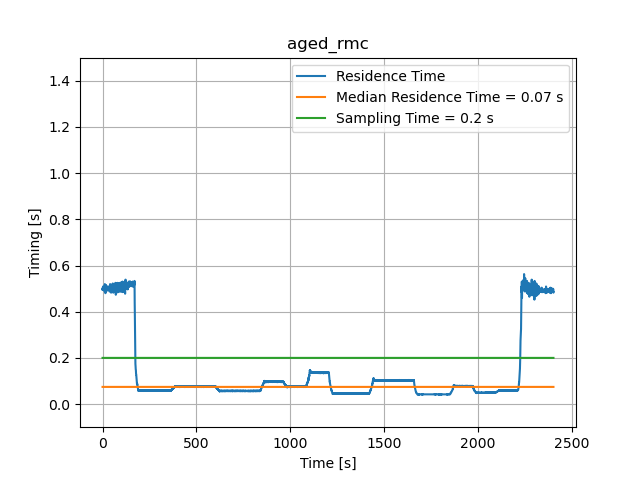
\includegraphics[width=\textwidth]{figs/res_time/aged_rmc_timing_stuff.png}
        \end{figure}
    \end{minipage}
    \begin{minipage}{0.49\textwidth}
        \begin{figure}[H]
            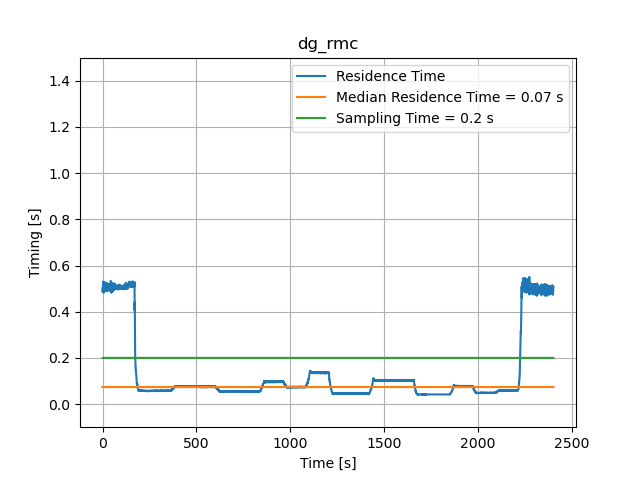
\includegraphics[width=\textwidth]{figs/res_time/dg_rmc_timing_stuff.png}
        \end{figure}
    \end{minipage}
    \begin{minipage}{0.49\textwidth}
        \begin{figure}[H]
            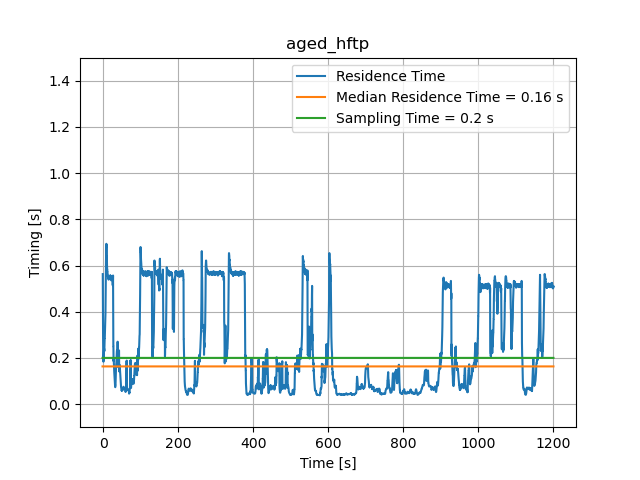
\includegraphics[width=\textwidth]{figs/res_time/aged_hftp_timing_stuff.png}
        \end{figure}
    \end{minipage}
    \begin{minipage}{0.49\textwidth}
        \begin{figure}[H]
            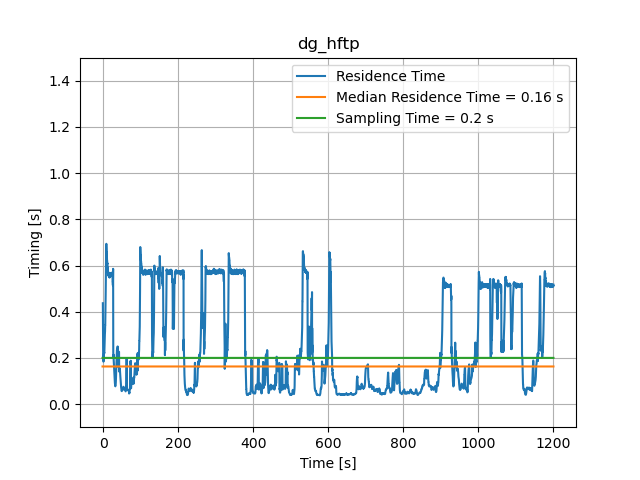
\includegraphics[width=\textwidth]{figs/res_time/dg_hftp_timing_stuff.png}
        \end{figure}
    \end{minipage}
    \begin{minipage}{0.49\textwidth}
        \begin{figure}[H]
            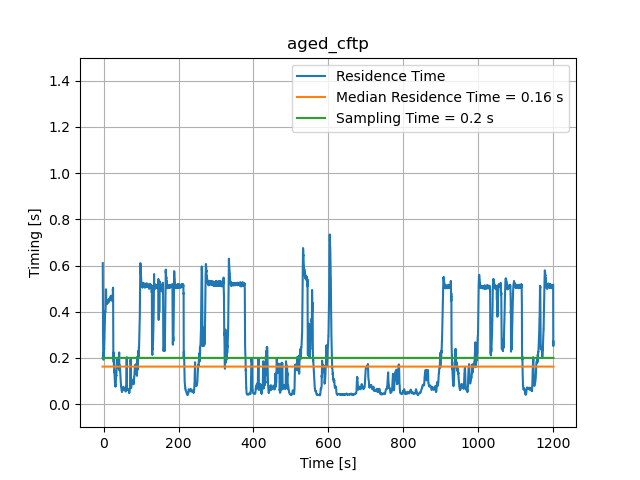
\includegraphics[width=\textwidth]{figs/res_time/aged_cftp_timing_stuff.png}
        \end{figure}
    \end{minipage}
    \begin{minipage}{0.49\textwidth}
        \begin{figure}[H]
            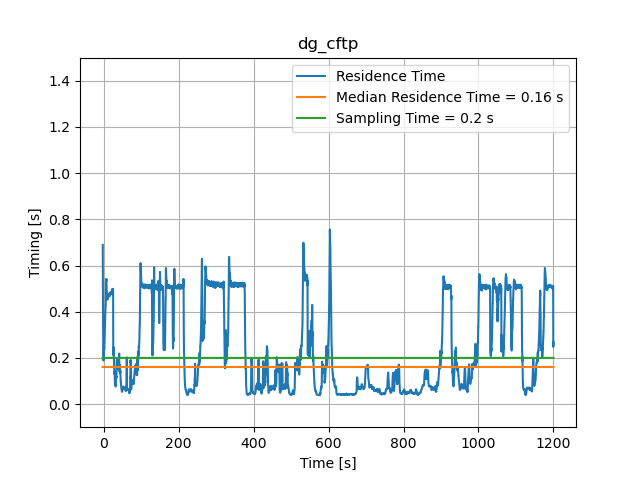
\includegraphics[width=\textwidth]{figs/res_time/dg_cftp_timing_stuff.png}
        \end{figure}
    \end{minipage}
\end{figure}


\subsubsection{Truck data}
\begin{figure}[H]
    \begin{minipage}{0.49\textwidth}
        \begin{figure}[H]
            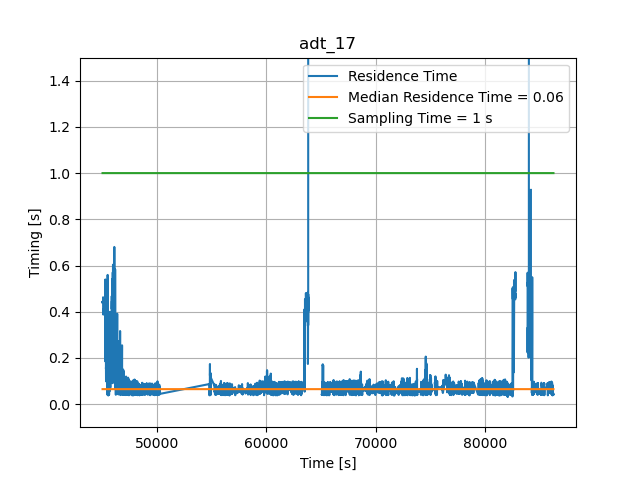
\includegraphics[width=\textwidth]{figs/res_time/adt_17_timing_stuff.png}
        \end{figure}
    \end{minipage}
    \begin{minipage}{0.49\textwidth}
        \begin{figure}[H]
            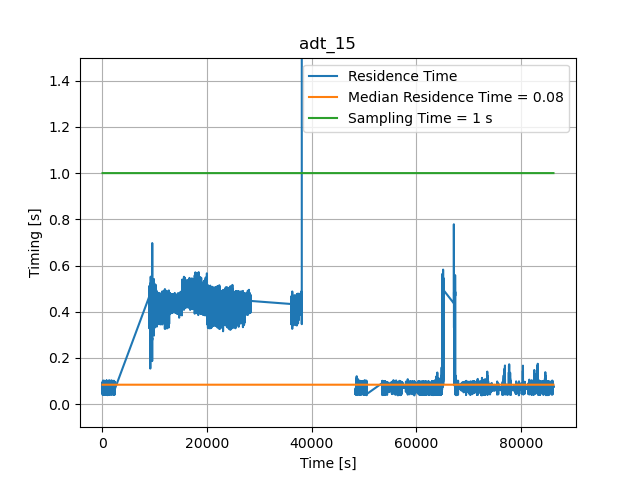
\includegraphics[width=\textwidth]{figs/res_time/adt_15_timing_stuff.png}
        \end{figure}
    \end{minipage}
    \begin{minipage}{0.49\textwidth}
        \begin{figure}[H]
            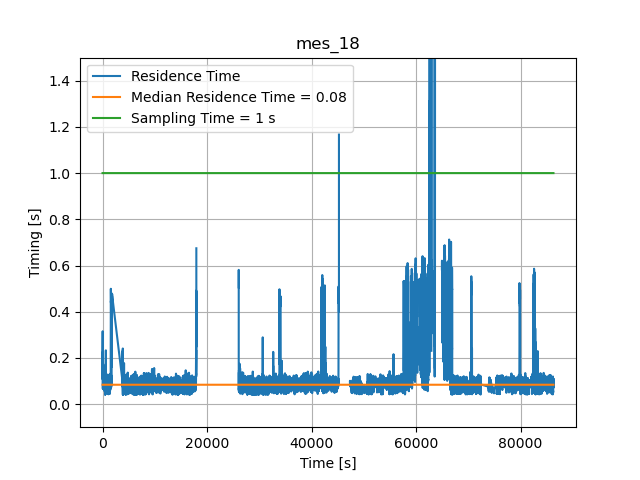
\includegraphics[width=\textwidth]{figs/res_time/mes_18_timing_stuff.png}
        \end{figure}
    \end{minipage}
    \begin{minipage}{0.49\textwidth}
        \begin{figure}[H]
            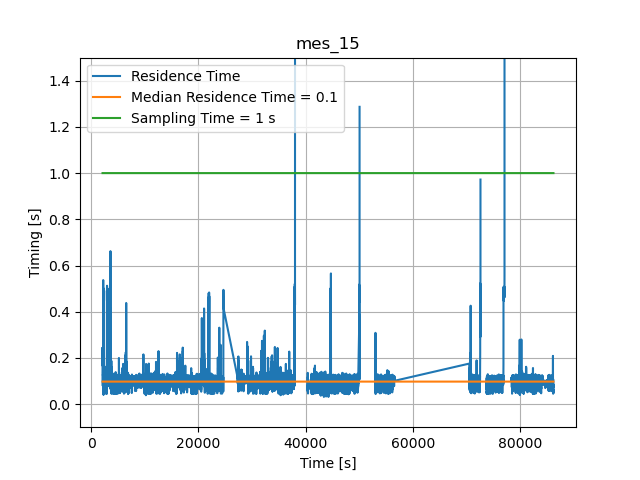
\includegraphics[width=\textwidth]{figs/res_time/mes_15_timing_stuff.png}
        \end{figure}
    \end{minipage}
    \begin{minipage}{0.49\textwidth}
        \begin{figure}[H]
            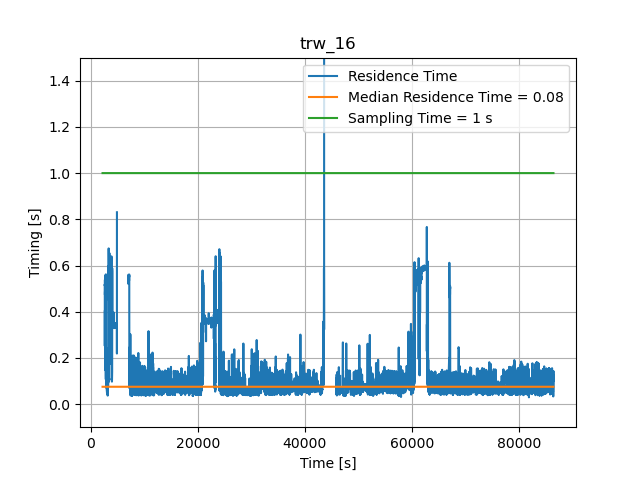
\includegraphics[width=\textwidth]{figs/res_time/trw_16_timing_stuff.png}
        \end{figure}
    \end{minipage}
    \begin{minipage}{0.49\textwidth}
        \begin{figure}[H]
            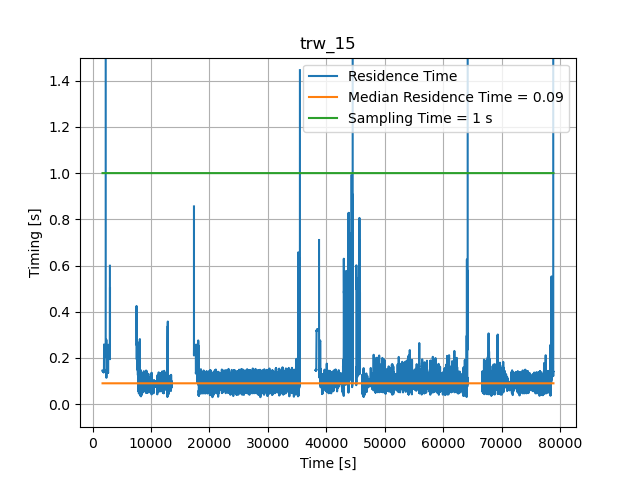
\includegraphics[width=\textwidth]{figs/res_time/trw_15_timing_stuff.png}
        \end{figure}
    \end{minipage}
\end{figure}
\begin{figure}[H]
    \begin{minipage}{0.49\textwidth}
        \begin{figure}[H]
            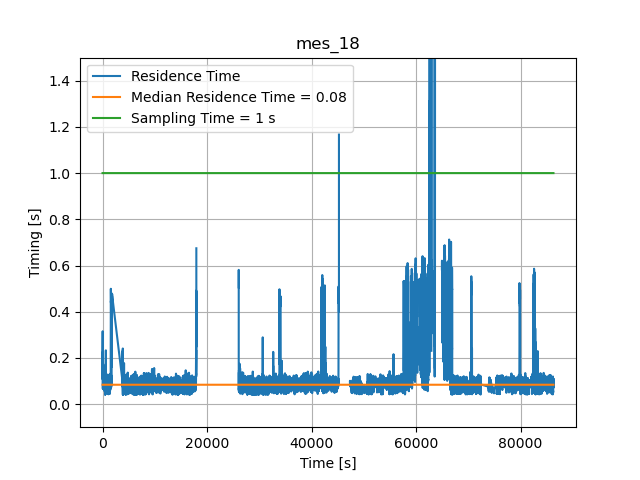
\includegraphics[width=\textwidth]{figs/res_time/mes_18_timing_stuff.png}
        \end{figure}
    \end{minipage}
    \begin{minipage}{0.49\textwidth}
        \begin{figure}[H]
            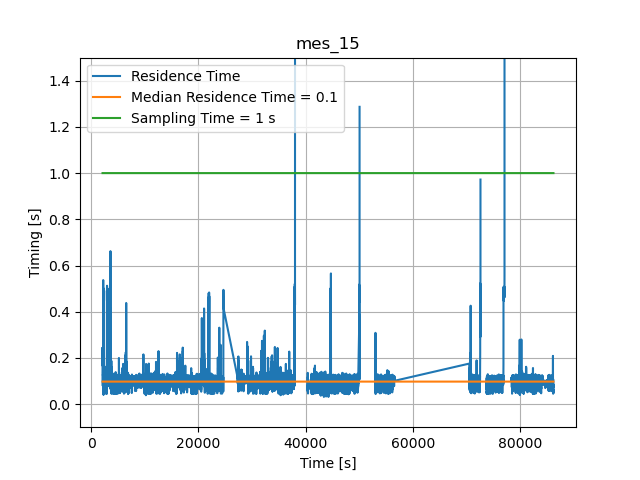
\includegraphics[width=\textwidth]{figs/res_time/mes_15_timing_stuff.png}
        \end{figure}
    \end{minipage}
\end{figure}

\subsection{Preliminary aging signature}
The $NO_x$ process dynamics can be rewritten as:
\begin{align*}
    \frac{\con{NO_x}^{in}(k) - \con{NO_x}^{out}(k + 1)}{\con{NO_x}^{in}(k)} &=
    k_{s2v} k_{scr} \sigma(k) \tau\\
    &= \frac{A_{scr}}{V} \times k_{scr} \times \sigma(k) \lr{\frac{V \rho}{F}}\\
    %===
    \implies F \lr{\frac{\con{NO_x}^{in}(k) - \con{NO_x}^{out}(k + 1)}{\con{NO_x}^{in}(k)}} &= \lr{\rho A_{scr} k_{scr}} \sigma(k) \\
    %===
\end{align*}

Using the linear assumption for temperature dependence of the rate constant, and
ideal gas-law for density, let:
\begin{align*}
    k_{scr} &= m_{scr} T + c_{scr}\\
    \rho &= \frac{\mu}{T}
\end{align*}
T is in Kelvin.
\begin{align*}
    \implies \underbrace{\lr{\mu A_{scr} m_{scr}}\sigma}_{\alpha_1(k)}  T+ \underbrace{\lr{\mu A_{scr} c_{scr}} \sigma}_{\alpha_0(k)} &= \underbrace{T F \lr{\frac{\con{NO_x}^{in}(k) - \con{NO_x}^{out}(k + 1)}{\con{NO_x}^{in}(k)}}}_{\beta(k)}
\end{align*}

Thus, $\alpha_1(k)$ and $\alpha_0(k)$ are monotonic first order
polynomials in $\sigma$. Assuming, the average surface concentration of ammonia
on the catalyst is higher for degreened catalyst than for aged catalyst, we can
use $\alpha_1, \alpha_0$ to define a preliminary aging signature for the
catalyst. This can be used to monitor the aging of the catalyst in real-time.


The variables, $\alpha_1(k)$ and $\alpha_0(k)$ change with time. The only way to
estimate these variables is to estimate a moving-averaged version of it.


% ==============================================================================
We have the above equation for $n$ (Averaging window) samples:

\begin{align*}
    \alpha_1(k) T(k) + \alpha_0(k) &= \beta(k)\\
    \alpha_1(k-1)T(k-1) + \alpha_0(k-1) &= \beta(k-1)\\
    \vdots &\\
    \alpha_1(k-(n-1))T(k-(n-1)) + \alpha_0(k-(n-1)) &= \beta(k-(n-1))\\
\end{align*}

Let,
\begin{align*}
    \bar \alpha_1(k) &= \frac{1}{n} \sum_{i=0}^{n-1} \alpha_1(k-i)\\
    \bar \alpha_0(k) &= \frac{1}{n} \sum_{i=0}^{n-1} \alpha_0(k-i)\\
\end{align*}

Thus, we have the following equation:
\begin{align*}
    \bm{\bar \alpha_1(k)\\
        \bar \alpha_0(k)} &=
        \bm{T(k) & 1\\
            T(k-1) & 1\\
            \vdots & \vdots\\
            T(k-(n-1)) & 1}^{-1}
        \bm{\beta(k)\\
            \beta(k-1)\\
            \vdots\\
            \beta(k-(n-1))}
\end{align*}


\end{document}
